\chapter{Upper and lower regularity dimensions}
\label{chap:upper_reg}


\section{Introduction}
\label{ch-upper-reg:intro-reg-dims}


This chapter aims to study some of the basic properties of the regularity dimensions. We investigate their relationship with familiar concepts such as the local dimensions, the $L^q$-spectrum, and weak tangents. Then we will explicitly calculate the dimensions of self-similar measures satisfying the strong separation property and self-affine measures supported on carpets and sponges satisfying the very strong separation property, which are some of the most standard examples of fractals. Finally the dimensions of measures on convergent sequences will be studied. These examples will exhibit several different types of behaviour and will demonstrate the sharpness of our general results. 


\section{Results regarding bounds and examples}\label{ch-upper-reg:results}

In this section we start by stating our results for the chapter. Bounds for the upper and lower regularity dimensions will be given in Section \ref{ch-upper-reg:bounds} whilst Section \ref{ch-upper-reg:sec:tangent} will study the dimensions of weak tangent measures. The regularity dimensions of self-similar and self-affine measures will be calculated in Sections \ref{ch-upper-reg:sec:self-similarresult} and \ref{ch-upper-reg:sec:self-affineresults}, respectively, whilst measures defined on certain sequences will be studied in Section \ref{ch-upper-reg:sec:sequences}. 

\subsection{General bounds}\label{ch-upper-reg:bounds}

The \textit{local dimensions} of a measure are the main tool for characterising the local scaling laws of a measure at small scales. The upper local dimension of $\mu$ at $x \in \text{supp}(\mu)$ is defined by
\nomenclature[dimlocal1]{$\ulocal$}{upper local dimension of $\mu$ at $x$}
\[
\ulocal=\limsup_{r\rightarrow 0} \frac{\log \mu(B(x,r))}{\log r}.
\]
The lower local dimension $\llocal$ is defined similarly by
\nomenclature[dimlocal2]{$\llocal$}{lower local dimension of $\mu$ at $x$}
\[
\llocal=\liminf_{r\rightarrow 0} \frac{\log \mu(B(x,r))}{\log r}.
\]
When these dimensions coincide we simply refer to the local dimension of the measure at $x$ and write $\dim_{\text{loc}}(x,\mu)$. These local dimensions clearly depend on the point $x$, but naturally give rise to dimensions depending only on $\mu$. For example, the lower Hausdorff dimension of $\mu$ is defined by
\[
\underline{\dim}_\H \mu=\text{ess}  \inf \left\{  \underline{\dim}_{\text{loc}}(x,\mu)  \ : \  x\in \text{supp}(\mu) \right\} 
\]
and the upper packing dimension is
\[
\overline{\dim}_\P \mu=\text{ess}  \sup \left\{ \overline{\dim}_{\text{loc}}(x,\mu) \ : \  x\in \text{supp}(\mu) \right\}.
\]
Recall, the essential supremum ($\text{ess} \sup$) is the supremum which holds for a set of full measure, similarly for the essential infimum. For instance the Hausdorff dimension of a measure is often written $$\underline{\dim}_\H \mu = \sup\left\{ s \ge 0 \colon \llocal \ge s  \text{ for $\mu$ almost all }x  \right\}.$$ 

A measure $\mu$ is called exact dimensional when $\underline{\dim}_\H \mu=\overline{\dim}_\P \mu$. It follows from the above definitions that in this situation, almost all points have the same local scaling behaviour. This provides a significant level of regularity which is often sufficient when studying the Hausdorff dimension. However this does not imply that all points satisfy the same power law, and so the regularity dimensions, which focus on extremal points, need further conditions to ensure equality.


There is a fairly straightforward relationship between the upper regularity dimension of a measure and the upper local dimensions. One can immediately obtain the following

\begin{lemma}
For any locally finite Borel measure $\mu$
\[
\r \geq \sup \left\{ \overline{\dim}_{\text{loc}}(x,\mu) \ : \  x\in \text{supp}(\mu) \right\}.
\]
\end{lemma} 
This shows that the upper regularity dimension is sensitive to large upper local dimension even at a single point.  

In particular, let $x \in \text{supp}(\mu)$ and let $s > \r$.  Then, by the definition of the upper regularity dimension, for small enough $r < R$ we have
\[
\frac{\mu(B(x,R))}{\mu(B(x,r))} \leq C\left(\frac{R}{r}\right)^{s}
\]
for some constant $C>0$.  Fixing $R$ and letting $r \to 0$ we obtain
\[
\overline{\dim}_{\text{loc}}(x,\mu)=\limsup_{r\rightarrow 0} \frac{\log \mu(B(x,r))}{\log r} \leq  \limsup_{r\rightarrow 0} \frac{\log \mu(B(x,R)) (r/R)^s/C }{\log r}  = s
\]
as required. 

This lower bound, combined with the Assouad dimension, gives a concrete and sometimes sharp lower bound on the upper regularity dimension. For example, we will show that for any self-similar measure $\mu$ satisfying the strong separation condition we have $ \r = \sup \left\{ \overline{\dim}_{\text{loc}}(x,\mu) \ : \  x\in \text{supp}(\mu) \right\}$.  However, for self-affine measures $\mu$, one may have
\[
\r >  \sup \left\{ \overline{\dim}_{\text{loc}}(x,\mu) \ : \  x\in \text{supp}(\mu) \right\}.
\]

Analogously, the lower regularity dimension of a measure $\mu$ can be related to the lower local dimensions by the following.
\begin{lemma}
For any locally finite Borel measure $\mu$ supported on a metric space $X$
\[
\lrdim \mu \le \inf \left\{\llocal \colon x \in \text{supp}(\mu) \right\}.
\]
\end{lemma}
Indeed, let $x\in \text{supp}(\mu)$ and $t < \lrdim \mu$. Then for any $r < R$ small enough we have
\[
\frac{\mu(B(x,R))}{\mu(B(x,r))} \geq C\left(\frac{R}{r}\right)^{t}
\]
for some constant $C$. Fixing $R$ and again letting $r \rightarrow 0$ gives
\[
\llocal = \liminf \frac{\log \mu(B(x,r)}{\log r} \ge t
\]
as desired.

A measure $\mu$ is Ahlfors-David $s$-regular if there exists constants $0<c_0,C_0< \infty$ such that 
\[
c_0 R^s \le \mu(B(x,R)) \le C_0 R^s
\]
for all $x\in \text{supp}(\mu)$ and $0 < R < \lvert \text{supp}(\mu) \rvert$.
These measures are even more regular than exact dimensional measures in that the ratio $\mu(B(x,R))/R^s$ is uniformly bounded away from 0 and $+\infty$ where $s >0$ is the `dimension'.  An Ahlfors-David $s$-regular measure is clearly exact dimensional (with exact dimension equal to $s$) and even satisfies $\lrdim \mu = \urdim \mu = s$. This provides the first concrete examples of measures where the local dimensions can recover the regularity dimensions. Note that equality of the regularity dimensions does not imply that the measure is Ahlfors-David regular, see \cite{hare-troscheit}.




We have already noted that the Assouad dimension of the support and the supremum of the upper local dimensions give elementary lower bounds for the upper regularity dimension.  We can refine this observation by further relating the upper regularity dimension to the \textit{(lower) $L^q$-spectrum}.  Let $\mu$ be a compactly supported probability measure on $\mathbb{R}^d$.  Given $q \in \mathbb{R}$ and $r>0$ we let
\nomenclature[d]{$d(\cdot, \cdot)$}{distance between two points in a metric space}
\[
M_r^q(\mu) = \sup  \, \left \{ \sum_{i=1}^\infty  \mu(B(x_i,r))^q \ : \ d(x_i, x_j) > 2r \text{ for $i \neq j$} \right\}
\]
be the multifractal packing function, see \cite{olsenformalism}.  The  (lower) $L^q$-spectrum of $\mu$ is then given by
\[
\underline{\tau}(q)= \liminf_{r\rightarrow 0} \frac{\log M_r^q(\mu) }{\log r}, \qquad (q\in \mathbb{R}).
\]
The $L^q$-spectrum gives a description of the global fluctuations of the measure and is a key tool in multifractal analysis, along with the multifractal spectrum. The \textit{multifractal spectrum} of $\mu$ is the function 
\[
f(\alpha) = \dim_\H \left\{ x\in \text{supp} (\mu) \colon \dim_{\textup{loc}}(x,\mu) = \alpha \right\}.
\]
For example, the Legendre transform of the $L^q$-spectrum is an upper bound for the multifractal spectrum of $\mu$ and, for measures satisfying the multifractal formalism, the Legendre transform of the $L^q$-spectrum is precisely the multifractal spectrum. Further information on the multifractal formalism can be found in \cite{olsenformalism} and the references therein. As such, one can bound the supremum of the upper local dimensions by the `top of the spectrum', defined by
\[
T(\mu)=\sup \left\{ s \ge 0 \colon \underline{\tau}(q) < sq \, \,, \forall q<0 \right\}
\]
which is the gradient of the asymptote to $\underline{\tau}(q)$ as $q \rightarrow - \infty$.  We prove that the upper regularity dimension is bounded below by the top of the spectrum.  


\begin{theorem} \label{ch-upper-reg:relationships}
	Given a compactly supported Borel probability measure $\mu$ on $\mathbb{R}^d$, we have
	\[
	\begin{array}{ccccccccccc}
	&&                  \sup_ {x\in \mathrm{supp}(\mu)}  \overline{\dim}_{\mathrm{loc}}(x,\mu)   \quad  \leq    \quad   T(\mu)                        & & &    \\
	&                       \rotatebox[origin=c]{45}{$\leq$}          & &              \rotatebox[origin=c]{315}{$\leq$} & &   \\
	\overline{\dim}_\text{\emph{P}} \mu                                            & &        &&                  & \r.\\
	&                \rotatebox[origin=c]{315}{$\leq$}              &&           \rotatebox[origin=c]{45}{$\leq$} & &  \\
	&&                                            \dim_\text{\emph{P}} \mathrm{supp}(\mu)      \quad  \leq   \quad  \dim_\text{\emph{A}} \mathrm{supp}(\mu)                           & & &  
	\end{array}
	\]
\end{theorem}

Most of the inequalities in the above theorem are well-known or have already been established above.  The only two remaining are the inequalities involving $T(\mu)$ and we prove these in Section \ref{ch-upper-reg:spectrumproof}. We take some inspiration from \cite{fraser-jordan} where the $L^q$-spectrum was related to the infimum of the lower local dimensions.


Expanding on the work of \cite{fraser-jordan}, combined with the above ideas, gives bounds relating the lower local dimension, the `lower end of the spectrum' and the lower regularity dimension. Formally, let the lower end of the spectrum be
\[
t(\mu) = \inf\left\{ s \ge 0 \colon \underline{\tau}(q) < sq  \, \,, \forall q<0 \right\}.
\]
Then the lower regularity dimension is bounded above by the lower end of the spectrum which is in turn always bounded above by the smallest local dimension.

\begin{theorem} \label{ch-upper-reg:lower-relationships}
	Given a compactly supported Borel probability measure $\mu$ on $\mathbb{R}^d$, we have
	\[
    \lrdim \mu  \le  t(\mu)  \le  \inf_ {x\in \mathrm{supp}(\mu)}  \underline{\dim}_{\mathrm{loc}}(x,\mu).
    \]
\end{theorem}
The proof of this Theorem will also be in Section \ref{ch-upper-reg:spectrumproof}. As with the upper regularity dimension, these notions can be linked to the lower and Hausdorff dimensions using known results. 

Many of the lower dimension results in this section were first proved in \cite{hare_troscheit}, including the relation between the lower regularity dimension and the infimum of the lower local dimensions. However the proofs used in this thesis will follow the ideas found in \cite{fraser-howroyd2} to ease comprehension.




\subsection{Weak tangent measures}\label{ch-upper-reg:sec:tangent}


One of the most powerful tools for providing lower bounds for the Assouad dimension of a set is the well-known result of Mackay and Tyson concerning weak tangents \cite[Proposition 6.1.5]{mackaytyson}. In particular, the Assouad dimension of any weak tangent to a set cannot exceed the Assouad dimension of the set itself. We state a slightly modified version of this result due to Fraser \cite[Proposition 7.7]{Fr}. 
\begin{proposition}[Very weak tangents]\label{ch-upper-reg:tangents}
Let $X\subset \mathbb{R}^d$ be compact and let $F$ be a compact subset of $X$. Let $(T_k)$ be a sequence of bi-Lipschitz maps defined on $\mathbb{R}^d$ with Lipschitz constants $a_k, b_k \ge 1$ such that 
\[
a_k d(x,y) \leq d( T_k(x) , T_k(y) ) \leq b_k d( x, y)  \,\,\,\,\,\,\,\, (x,y\in\mathbb{R}^d),
\]
where
\[
\sup_k b_k / a_k = C_0 <\infty
\]
and suppose that $T_k(F) \cap X \rightarrow \hat{F}$ in the Hausdorff metric. Then the set $\hat F$ is called a \emph{very weak tangent} to $F$ and, moreover,  $\dim_{\text{\emph{A}}} F \geq \dim_{\text{\emph{A}}} \hat{F}$.
\end{proposition}
The Hausdorff distance between two subsets $X,Y$ of $\mathbb{R}^d$ is defined by
\[
d_{\mathcal{H}}(X,Y) = \max\left\{\sup_{x\in X} \inf_{y \in Y} d(x,y), \sup_{y\in Y} \inf_{x \in X} d(x,y)\right\}.
\]
\nomenclature[d]{$d_{\mathcal{H}}(\cdot, \cdot)$}{Hausdorff distance between two sets}


These weak tangents are often called microsets, as first defined by Furstenberg in the 60s \cite{furstenberg70, furstenberg}, and have been fundamental in the study of the Assouad dimension. This includes aiding direct calculations of the dimension of sets as in \cite{fraser-howroyd1}, the direct relationship between the dimensions of microsets and the Assouad dimension as in \cite{kaenmaki-assouad, microsets} and even linking fractal geometry with number theory and the Erd\"os-Tur\'an conjecture in \cite{FY}. A result similar to Proposition \ref{ch-upper-reg:tangents} holds for the lower dimension and the smallest tangent sets with some added conditions; these additions were first introduced in \cite{Fr} but are not needed in the measure setting.


\nomenclature[mu2]{$\hat{\mu}$}{weak tangent measure of $\mu$}
\nomenclature[R]{$\mathbb{R}$}{the reals}
Given that the upper regularity dimension is the `Assouad dimension of a measure', it is natural to consider a result analogous to Proposition \ref{ch-upper-reg:tangents} in the setting of measures, where we replace convergence in the Hausdorff metric with weak convergence of measures. A sequence of positive probability measures $\left\{\mu_n\right\}_{n\in \mathbb{N}}$ supported on subsets of a space $X$ is said to weakly converge to another measure $\mu$ also supported on a subset of $X$ if $\int fd \mu_n \rightarrow \int fd \mu$ as $n\rightarrow \infty$ for all continuous functions $f\colon X \rightarrow \mathbb{R}$. We then say that a measure  $\hat{\mu}$ on $ \mathbb{R}^d$ is a \emph{weak tangent measure} to a locally finite measure $\mu$ on $\mathbb{R}^d$ if there exists a sequence of similarity maps $T_k$ on  $\mathbb{R}^d$ and a sequence of positive re-normalising numbers $p_k$ such that
\[
p_k \mu \circ T^{-1}_k  \rightharpoonup \hat{\mu}
\]
\nomenclature[.]{$\rightharpoonup$}{weak convergence of measures}
where $\rightharpoonup$ denotes weak convergence. Recall that a map $T$ on $\mathbb{R}^d$ is a \emph{similarity} if there is a constant $c  \in \left(0,1 \right)$ such that  for all $x,y \in \mathbb{R}^d$ we have $d(T(x) , T(y) ) = c \, d(x, y )$.  We refer to $c$ as the \emph{similarity ratio}. 

\emph{Tangent measure} usually refers to a weak limit of magnifications of a given measure at a specific point, in contrast to weak tangent measures where the point of magnification can move around. In the seminal work of Preiss \cite{preiss} tangent measures were allowed to have unbounded support and when one restricts the magnifications to a fixed compact set, the (compactly supported) limit measures are often called \emph{micromeasures}, following the important work of Furstenberg \cite{furstenberg} and Hochman \cite{hochman}.  


\begin{theorem}\label{ch-upper-reg:weaktangents}
	Suppose $\hat{\mu}$ is a weak tangent measure to a locally finite Borel measure  $\mu$ on $\mathbb{R}^d$.  Then 
	\[\overline{\dim}_{\textup{reg}} \hat{\mu} \le \r \]
	and
	\[\lrdim \hat{\mu} \ge \lrdim \mu.	\]
\end{theorem}

We will prove this result in Section \ref{ch-upper-reg:weaktangentsproof}.  An immediate corollary  is that weak tangent measures of doubling measures are doubling.  This observation generalises the folklore result that `tangent measures of doubling measures are doubling'. Similarly for uniformly perfect measures. 

\begin{corollary}
	All weak tangent measures of doubling measures are doubling. All weak tangent measures of uniformly perfect measures are uniformly perfect.
\end{corollary}



In our definition of weak tangent measures we follow the strategy of Preiss, allowing the tangent to have unbounded support. However the weak tangent (sets) for Assouad dimension follow the conventions of Furstenberg and Hochman, restricting to a compact set. It turns out that this difference in approach is necessary as the dimension of a set cannot increase under restriction but the dimension of a measure can. The general problem of determining when a doubling measure restricts to a doubling measure on a compact set of positive mass is a subtle problem, see \cite{ojala}.  We provide a simple example of a doubling measure on the plane which, upon restriction to the unit ball, becomes non-doubling.  In particular this shows that if, in the definition of weak tangent measures, one restricts the measures $p_k \mu \circ T^{-1}_k$ to the unit ball, the analogue of Theorem \ref{ch-upper-reg:weaktangents} generally fails. This is because the restricted measure would become a weak tangent measure to the original measure.

We begin with the square $X_0 = [-3/2, 3/2]^2$ and cut out a sequence of open   `almost' semicircles as follows.   Let $\left\{r_i \right\}_{i\in \mathbb{N}}$ be a sequence of radii which decay exponentially to 0 and $\left\{x_i\right\}_{i\in \mathbb{N}}$ be a sequence of centres moving clockwise on  $S^1$ which converge polynomially to a limit on the opposite side of $S^1$ from $x_1$ (without making any full rotations). Consider the balls $B_i = B(x_i, r_i)$ and remove from $X_0$ the points in the interior of  $B_i \cap B(0,1)$ which are at distance strictly greater than $r_i^2$ from $S^1$, see the portion shown in grey on the left in Figure \ref{ch-upper-reg:example}.  After all of these portions have been removed, label the remaining set as $X$.  The complement of $X$ is shown in grey on the right of Figure \ref{ch-upper-reg:example}. 

\begin{figure}[h]
	\centering
	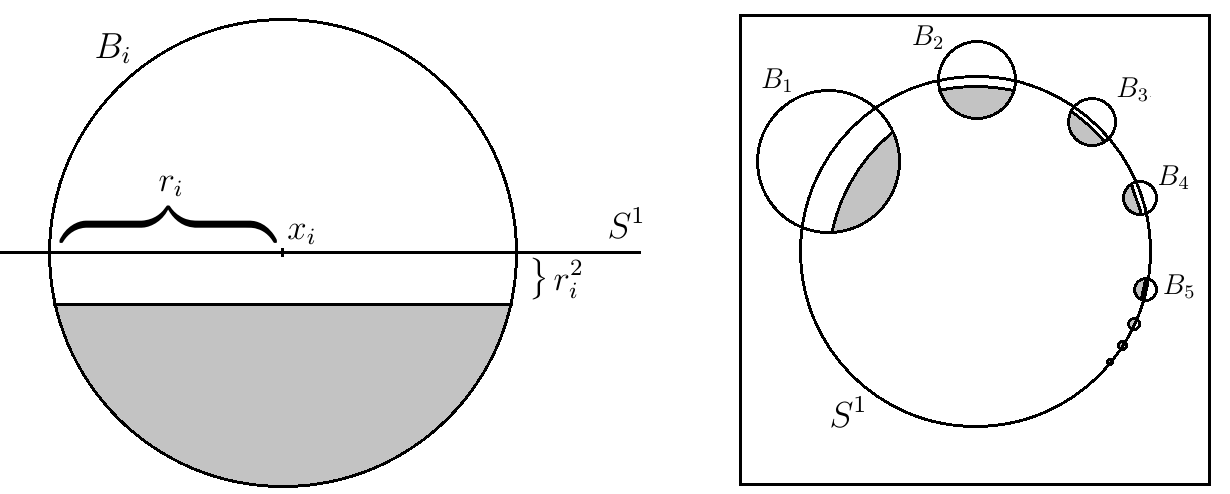
\includegraphics[width=0.9\textwidth]{pics/ch-upper-reg/example.png}
	\caption{Construction of a doubling measure which is not doubling after restricting to the unit ball}
	\label{ch-upper-reg:example}
\end{figure}

We observe  that 2-dimensional Lebesgue measure $\mu$ on $X$ is doubling, but that the restriction of $\mu$ to $B(0,1)$ is not doubling.  It is easy to see that there exists a uniform constant $c>0$ such that for $x \in X$ and $r\in (0,1)$ we have $cr^2 \leq \mu(B(x,r)) \leq \pi r^2$.  It follows that $\mu$ is doubling (with upper regularity dimension 2).  We now consider the restricted measure $\nu = \mu \vert_{B(0,1)}$ and compare the masses of $B(x_i,r_i)$ and $B(x_i,2r_i)$. For large enough $i$ we have $\nu (B(x_i,2r_i)) \ge (\pi (2r_i)^2-\pi r_i^2)/3 = \pi r_i^2$  and $\nu (B(x_i,r_i)) \le 4 r_i^3$. Therefore
\[
\frac{\nu(B(x_i,2r_i))}{\nu(B(x_i,r_i))} \ge \frac{\pi r_i^2}{4r_i^3} =  \frac{\pi}{4r_i} \to \infty
\]
and so  $\nu$ is not doubling.


\subsection{Self-similar measures}\label{ch-upper-reg:sec:self-similarresult}

In this section we compute the regularity dimensions of self-similar measures satisfying the strong separation condition. We emphasise that this separation assumption is natural because self-similar measures not satisfying the strong separation condition are typically not doubling and so have upper regularity dimension equal to $+\infty$. An example of this behaviour is provided below when the strong separation condition is formally defined. 

\nomenclature[IFS1]{IFS}{iterated function system}
\nomenclature[IFS2]{$\mathcal{I}$}{finite index set for an iterated function system}
Let  $\mathcal{I}$ be a finite index set and $\left\{S_i \right\}_{i \in \mathcal{I}}$ be a finite collection of  contraction maps on a compact subset of $\mathbb{R}^d$.  Such a collection is known as an \textit{iterated function system} (IFS).  Also let $\{p_i\}_{i \in \mathcal{I}}$ be a collection of probabilities associated with the maps $\{S_i\}_{i \in \mathcal{I}}$, i.e. we assume that for each $i \in \mathcal{I}$ we have $p_i>0$ and $\sum_{i \in \mathcal{I}} p_i = 1$. There is a  unique non-empty compact set $F$ satisfying 
\[
F=\displaystyle\bigcup_{i\in \mathcal{I}} S_i(F)
\]
and  a unique Borel probability measure $\mu$ satisfying
\[
\mu = \sum_{i \in \mathcal{I}} p_i \mu \circ S_i^{-1}
\]
which is fully supported on $F$, see \cite[Chapter 9]{falconer} and the references therein, notably \cite{hutchinson}. When all of the contractions $S_i$ are similarities, with similarity ratio $c_i \in \left(0,1 \right)$, then $F$ is called a \emph{self-similar set} and $\mu$ is called a \emph{self-similar measure}. These sets are some of the most well studied examples of fractals yet there are many subtleties that we still do not understand, a recent example is \cite{baker}. We refer the reader to \cite{falconer} for a more in depth discussion of IFSs and self-similar sets and measures.

\begin{figure}[h]
	\centering
	\begin{subfigure}{0.3\textwidth}
		\centering
		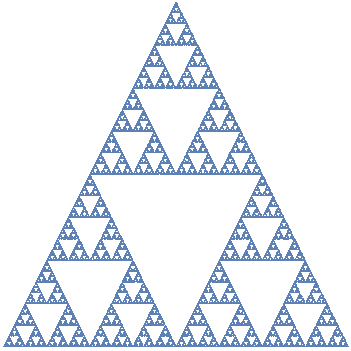
\includegraphics[width=0.85\linewidth]{pics/ch-upper-reg/sierp.png}
	\end{subfigure}%
	\begin{subfigure}{.3\textwidth}
		\centering
		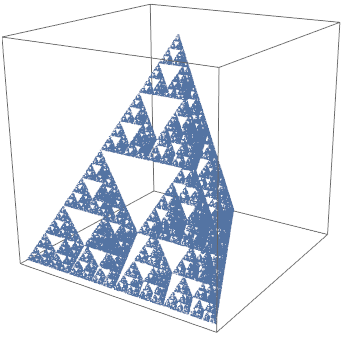
\includegraphics[width=.9\linewidth]{pics/ch-upper-reg/sierptetra.png}
	\end{subfigure}%
	\begin{subfigure}{.3\textwidth}
		\centering
		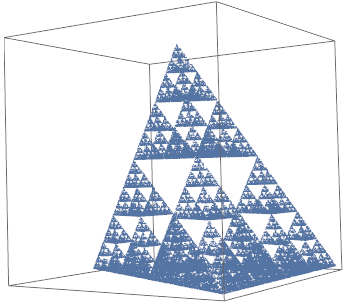
\includegraphics[width=.9\linewidth]{pics/ch-upper-reg/sierptetra2.png}
	\end{subfigure}
	\caption{A self-similar Sierpi\'nski triangle and two perspectives of a self-similar Sierpi\'nski tetrahedron}
	\label{ch-upper-reg:fig:test}
\end{figure}

\nomenclature[SSC]{SSC}{strong separation condition}
We say that the IFS (and associated set $F$ and measure $\mu$) satisfy the \emph{strong separation condition (SSC)} if $S_i(F) \cap S_j(F) = \emptyset$ for all distinct $i,j \in \mathcal{I}$.  This is a natural assumption in the context of the upper regularity dimension. For example, if the defining IFS consists of the maps $x \mapsto x/2$ and $x \mapsto x/2+1/2$, then the SSC is not satisfied and one easily verifies that $\mu$ is doubling if and only if both probabilities are equal to 1/2 and in this case $\mu$ is Ahlfors-David 1-regular (it is Lebesgue measure on the unit interval). On the other hand, when the strong separation condition does not hold, measures can still have positive, even maximal lower regularity dimension; we do not pursue this here and direct the reader towards \cite{hare-troscheit} for further elaboration.  

It is a classical result due to \cite{hutchinson} that the Hausdorff dimension of a self-similar set satisfying the strong separation condition and with contractions $\left\{c_i \right\}_{i\in \lambda}$ is the unique $s$ satisfying $\sum_{i\in \Lambda} c_i^s = 1$. In fact, these sets are incredibly regular so the box, Assouad and lower dimensions are all equal to the Hausdorff dimension. As we weaken the separation condition these numbers start to differ in a number of cases. Studying such cases has seen huge advances recently, as in \cite{hochman2}. The Hausdorff dimension of self-similar measures on self-similar sets satisfying the SSC is known to be $\underline{\dim}_{\textup{H}} \mu = \sum p_i \log p_i / \sum p_i\log c_i$ and these measures are exact dimensional. In this setting the multifractal formalism is satisfied and formulae for the ends of the spectrum can be found in \cite{cawley-mauldin, olsenformalism}.

The regularity dimensions do not behave quite as nicely as one might hope in this setting in the sense that they do not equal the Hausdorff dimension of the measure. However, they do interact pleasantly with the multifractal spectrum of the measure.

\begin{theorem}\label{ch-upper-reg:selfsimilar}
	Let $\mu$ be a self-similar measure as defined above and assume $\mu$ satisfies the SSC.  Then 
	\[
	\urdim \mu = \sup_x \overline{\dim}_{\textup{loc}}(x,\mu) = T(\mu) = \max_{i \in \mathcal{I}} \frac{\log p_i}{\log c_i}
	\]
	and 
	\[
	\lrdim \mu = \inf_x \overline{\dim}_{\textup{loc}}(x,\mu) = t(\mu) = \min_{i \in \mathcal{I}} \frac{\log p_i}{\log c_i}
	\]
\end{theorem}

The Assouad dimension of the self-similar set which supports $\mu$ is generally strictly smaller than the upper regularity dimension of $\mu$ in this setting.  In fact the only case where the geometric dimension and corresponding measure dimension coincide is when  $p_i=c_i^s$, where $s$ is the Hausdorff dimension of the set. In this case $\mu$ is Ahlfors-David $s$-regular and all of the notions of dimension for $F$ and $\mu$ coincide and equal $s$.

\begin{figure}[htb]
    \centering
    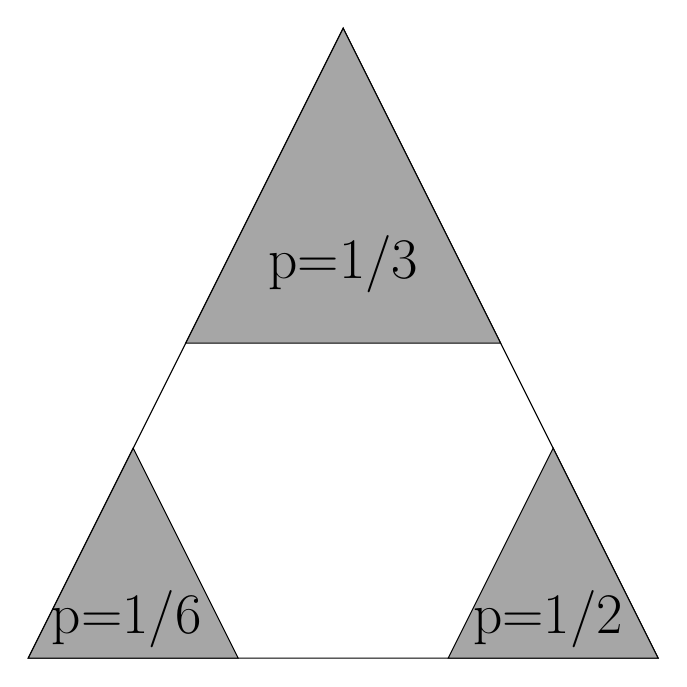
\begin{tikzpicture}
\draw (0,0) 
  -- (8,0) 
  -- (4,8) 
  -- cycle;

\draw[black,fill=gray!70] (0,0)
  -- (4/3,8/3) 
  -- (8/3,0) 
  -- cycle;
\draw[black,fill=gray!70] (16/3,0) 
  -- (20/3,8/3) 
  -- (8,0) 
  -- cycle;
\draw[black,fill=gray!70] (4,8)  
  -- (2,4)
  -- (6,4) 
  -- cycle;

\node at (1.25,0.5) {\huge p=1/6};
\node at (6.6,0.5) {\huge p=1/2};
\node at (4,5) {\huge p=1/3};
\end{tikzpicture}
    \caption{First step in the construction of a self-similar set satisfying the SSC and an associated measure}
    \label{fig:ex-self-sim}
\end{figure}



The figure above is the first stage in the construction of a self-similar set in $2$ dimensions with 3 maps $f_1, f_2$ and $f_3$ of respective contraction ratios $1/3$, $1/3$ and $1/2$ and associated probabilities $1/6$, $1/2$ and $1/3$. The attractor $F$ of this IFS satisfies the strong separation condition so the main dimensions all coincide and equal
\[
\dim_\H F = \dim_\textup{B} F = \Assouad F = \lowerdim F \approx 1.17.
\]
The probability vector and the IFS define a self-similar measure $\mu$. The previously discussed dimensions of measures are distinct for this measure with
\[
\underline{\dim}_\H \mu = \frac{4 \log 2 + 3 \log 3}{2 \log 2 + 4 \log 3} \approx 1.05,
\]
\[
\urdim \mu = \frac{\log 6}{\log 3} \approx 1.63
\]
and 
\[
\lrdim \mu = \frac{\log 2}{\log 3} \approx 0.63.
\]


In this section we restricted attention to self-similar sets satisfying the strong separation condition, whilst certain overlap conditions have been covered in \cite{hare-hare-tros} and others are already known, it is always of interest to extend to the most general setting possible.
\begin{question}
What are the regularity dimensions of self-similar measures on sets not satisfying the strong separation condition?
\end{question}





\subsection{Self-affine measures}\label{ch-upper-reg:sec:self-affineresults}


In this section we consider an important class of self-affine measures.  Self-affine measures are defined in a similar way to the self-similar measures considered in the previous section, the only difference being that the defining contractions are assumed to be affinities rather than similarities.  In general, such measures are much more difficult to handle due to the fact that different rates of distortion can occur in different directions.  The specific class of self-affine measures we consider are those supported on Bedford-McMullen carpets, see \cite{bedford, mcmullen}, and on the higher dimensional analogues, Bedford-McMullen sponges, see \cite{kenyonperes, sponges}. 

The study of self-affine sets can be broken into two parts: the study of general self-affine sets and specific examples such as Bedford-McMullen carpets. The generic case dates back to Falconer \cite{falconer-affine} where the affinity dimension was first defined. This case has seen a great deal of study recently as in \cite{barany-hochman-rapaport,hochman-rapaport}. On the other hand, studying specific examples has seen a number of different results, including \cite{bedford,mcmullen, lalley-gatzouras, baranski, mackay, Fr}. In particular there is interest in understanding how the special cases, such as carpets, differ from the generic results, see \cite{jurga-morris, morris-sert}. 

\begin{figure}[h]
	\centering
	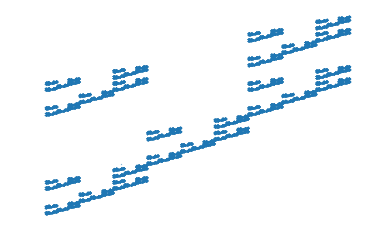
\includegraphics[width=0.8\linewidth]{pics/ch-upper-reg/self-affine-ex.png}
	\label{ch-upper-reg:fig:example-self-affine}
	\caption{An example of a Bedford-McMullen carpet with a 3 by 4 grid and 5 maps}
\end{figure}


Sponges (and measures defined on them) are less commonly studied, but came to prominence recently when they were used by Das and Simmons to provide a counter example to an important and long-standing conjecture in dynamical systems \cite{das-simmons}. In particular, there exists a surprising example of a sponge in $\mathbb{R}^3$ whose Hausdorff dimension cannot be approximated by the Hausdorff dimension of measures invariant under the natural associated dynamical system. This contrasts with the well known result of \cite{kaenmaki-affine} which states that an ergodic invariant measure can be found for typical self-affine sets so that the Hausdorff dimensions coincide.


Let $d \geq 2$ be an integer and fix integers $1<n_1 < n_2 \cdots < n_d$.  Choose a subset $\mathcal{I}$ of $\prod_{l=1}^{d} \left\lbrace 0,\ldots, n_l-1 \right\rbrace$ and for $\textbf{i}=(i_1, \ldots, i_d)\in \mathcal{I} $  let $S_{\textbf{i}} \colon [0,1]^d \rightarrow [0,1]^d$ be defined by
\[
S_{\textbf{i}}(x_1,x_2\ldots, x_d)= \left( \frac{x_1+i_1}{n_1}, \frac{x_2+i_2}{n_2}, \ldots, \frac{x_d+i_d}{n_d} \right) .
\]
Finally, consider the IFS $\{S_i\}_{i \in \mathcal{I}}$  acting on $[0,1]^d$ and let $\{p_i\}_{i \in \mathcal{I}}$ be an associated probability vector as before.  Let $F$ be the associated attractor of this IFS, which is a self-affine set since each of the defining contractions is an affinity, and let $\mu$ be the associated self-affine measure. 



We can now state the separation condition we require, which we note is strictly stronger than the SSC.

\nomenclature[VSSC]{VSSC}{very strong separation condition}
\begin{definition}[VSSC, \cite{sponges}]
	\emph{A self-affine sponge }$F$\emph{ (associated to an index set }$\mathcal{I}$)\emph{ satisfies the }very strong separation condition (VSSC)\emph{ if the following condition  holds. If }$l \in  \left\{1, \ldots, d\right\}$\emph{ and }$(i_1, \ldots, i_d)$, $(j_1 ,\ldots, j_d)\in \mathcal{I}$\emph{ satisfy }$i_1=j_1, \ldots,  i_{l-1}=j_{l-1}$\emph{ and }$i_l \neq j_l$,\emph{ then }$\lvert i_l - j_l \rvert >1$.
\end{definition} 


We assume the self-affine sets studied here satisfy the \emph{very strong separation condition}, which was used by Olsen in \cite{sponges}. Again, this is the natural condition to assume in the context of regularity dimensions because without this assumption the self-affine measures tend not to be doubling, see \cite{doublingcarpets, fraser-howroyd1}. 

\begin{figure}[h]
	\centering
	\begin{subfigure}{0.35\textwidth}
		\centering
		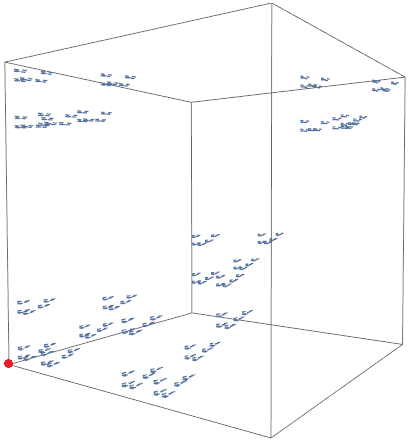
\includegraphics[width=0.8\linewidth]{pics/ch-upper-reg/sponge11.png}
		\label{ch-upper-reg:fig:sub1}
	\end{subfigure}%
	\begin{subfigure}{0.35\textwidth}
		\centering
		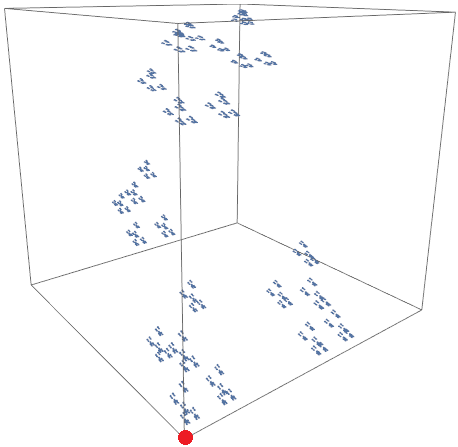
\includegraphics[width=0.85\linewidth]{pics/ch-upper-reg/sponge12.png}
		\label{ch-upper-reg:fig:sub2}
	\end{subfigure}%
	\begin{subfigure}{0.35\textwidth}
		\centering
		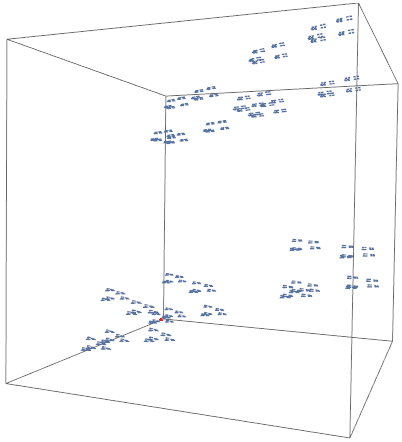
\includegraphics[width=0.85\linewidth]{pics/ch-upper-reg/sponge13.png}
		\label{ch-upper-reg:fig:sub2}
	\end{subfigure}
	\caption{Three perspectives of the self-affine sponge defined by the data: $d=3$,  $n_1=3$, $n_2=4$, $n_3=5$ and $\mathcal{I} = \{ (0,0,0),(0,2,0),(2,1,1)$, $(2,3,4)$, $(0,0,4) \}$. The origin is marked by a red dot to indicate orientation}
\end{figure}


Before we state our result, we need to introduce some more notation.  For $l=1, \dots, d$ and $\textbf{i}=(i_1, \ldots, i_d)\in \mathcal{I} $  let 
\[
p_l(\mathbf{i})=p (i_l \vert i_1, \ldots , i_{l-1})=\frac{\displaystyle\sum_{\substack{\textbf{j}=\left( j_1, \ldots, j_d\right)\in \mathcal{I} \\ j_1=i_1, \ldots, j_{l-1}=i_{l-1}, j_l=i_l}}p_{\textbf{j}}}{\displaystyle\sum_{\substack{\textbf{j}=\left( j_1, \ldots, j_d\right)\in \mathcal{I} \\ j_1=i_1, \ldots, j_{l-1}=i_{l-1}}}p_{\textbf{j}}}
\]
if $(i_1, \ldots, i_l, i_{l+1},\ldots, i_d) \in \mathcal{I}$ for some $i_{l+1},\ldots, i_d$ and $0$ otherwise.  These numbers have a clear interpretation: $p_l(\mathbf{i})$ is the conditional probability that the $l$th digit of an element of $\mathcal{I}$  coincides with the $l$'th digit of $\mathbf{i}$, given that the first $l-1$ coordinates did.  Note that when $l=1$ we are conditioning on the entire space and so the denominator of the above conditional probability is taken to be 1.

\newpage
\begin{theorem}\label{ch-upper-reg:carpet}
	Let $\mu$ be a self-affine measure on a Bedford-McMullen sponge satisfying the VSSC.  Then
	\[
	\urdim \mu =\sum_{l=1}^d \max_{\mathbf{i}\in \mathcal{I}}\frac{-\log p_l(\mathbf{i})}{\log n_l}
	\]
	and 
	\[
	\lrdim \mu =\sum_{l=1}^d \min_{\mathbf{i}\in \mathcal{I}}\frac{-\log p_l(\mathbf{i})}{\log n_l}.
	\]
\end{theorem}

For comparison, we will briefly consider the other notions of dimensions of Bedford-McMullen carpets, restricting to the two dimensional case for ease of notation. Let $N$ be the total number of maps in the IFS and for each column $i\in \left\{0,\ldots, n_1 - 1\right\}$ we define $N_i$ to be the number of maps in that specific column. Finally let $N^0$ to be the total number of non-empty columns. The Hausdorff and box dimensions of Bedford-McMullen carpets $F$ are 
\[
\dim_{\textup{B}} F = \frac{\log N^0}{\log n_1} + \frac{\log N/N^0}{\log n_2}
\]
and 
\[
\dim_{\textup{H}} F = \frac{\log \sum_{i=0}^{n_1 - 1} N_i^{\log n_1 / \log n_2} }{\log n_1}.
\]
The Assouad dimension of these sets was first calculated by Mackay in \cite{mackay}, whilst the lower dimension is due to Fraser in \cite{Fr}, and they are
\[
\Assouad F = \frac{\log N^0}{\log n_1} + \max_{i = 0, \ldots, n_1-1} \frac{\log N_i}{\log n_2}
\]
and 
\[
\lowerdim F = \frac{\log N^0}{\log n_1} + \min_{i = 0, \ldots, n_1-1} \frac{\log \max\{N_i, 1 \}}{\log n_2}.
\]
Note the lower dimension has a $\max\{N_i, 1\}$ in the second fraction, this is to prevent well definededness issues when a column is empty so $N_i \neq 0$.


Formulae for the local dimensions $\sup_x \overline{\dim}_{\text{loc}}(x,\mu), \inf_x \underline{\dim}_{\text{loc}}(x,\mu)$ and spectrum $T(\mu), t(\mu)$ for the self-affine measures $\mu$ we consider in this section can be found in \cite{sponges}, where the notation $\overline{a}, \underline{a}$ and $\overline{A}, \underline{A}$ was used, respectively.


We will now discuss a family of examples designed to demonstrate that all of the notions of dimension we discuss here can be distinct for self-affine measures.  In particular, the upper regularity dimension can be strictly greater than the Assouad dimension, supremum of the upper local dimensions and the `top of the spectrum', $T(\mu)$; similarly for the lower regularity dimension analogues.  This behaviour was \emph{not} seen in the self-similar case.

Let $d=2$, $n_1=3$, $n_2=4$,  $\mathcal{I}=\left\{(0,2),(2,1),(2,3)\right\}$ and $p_{(0,2)}=\epsilon,\, p_{(2,1)}=1-3\epsilon/2$ and $p_{(2,3)}=\epsilon/2$ where we allow $\epsilon$ to vary in the interval $(0,1/2]$.  We write $F$ for the self-affine carpet and $\mu$ for the self-affine measure associated with this data.  Observe that the VSSC is satisfied and so our results apply.  Theorem \ref{ch-upper-reg:carpet} yields
\[
\r = \frac{-\log \epsilon}{\log 3}+ \frac{-\log \frac{\epsilon/2}{1-\epsilon} }{\log 4}
\]
and 
\[
\lrdim \mu = \frac{-\log (1 - \epsilon)}{\log 3}.
\]
Mackay's and Fraser's results give
\[
\dim_{\text{A}} F = \frac{\log 2}{ \log 3} + \frac{ \log 2}{ \log 4} 
\]
and 
\[
\dim_{\text{L}} F = \frac{\log 2}{ \log 3}. 
\]
Olsen gives us
\[
\sup_{x\in F} \overline{\dim}_{\text{loc}}(x,\mu)=\max\left\{ \frac{-\log \epsilon}{\log 3} , \frac{-\log (1-\epsilon)}{\log 3}+\frac{-\log \frac{\epsilon/2}{1-\epsilon} }{\log 4}\right\},
\]
(which has a phase transition at $\epsilon \approx 0.066$),
\[
\inf_{x\in F} \underline{\dim}_{\text{loc}}(x,\mu)=\min\left\{ \frac{-\log \epsilon}{\log 3} , \frac{-\log (1-\epsilon)}{\log 3}+\frac{-\log \frac{1-3\epsilon/2}{1-\epsilon} }{\log 4}\right\},
\]
\[
T(\mu)= \frac{-\log \epsilon }{\log 3} +\frac{\log 2}{\log 4}
\]
and
\[
t(\mu)= \frac{-\log 1- \epsilon }{\log 3} +\frac{\log \frac{2(1-\varepsilon)}{1-3\varepsilon/2} }{\log 4}. 
\]
For $\epsilon \in (0,1/2)$  these quantities are all distinct and for $\epsilon=1/2$ the measure is the `coordinate uniform measure' from \cite{fraser-howroyd1} which has upper regularity dimension precisely equal to the Assouad dimension and lower regularity dimension equal to the lower dimension. This means the larger notions then become all equal and the lower concepts are also all the same, however the lower dimension is strictly less than the Assouad dimension so there is still a gap between them all.



\begin{figure}[H]
	\centering
	\begin{minipage}{.5\textwidth}
		\centering
		\begin{tikzpicture}[scale=0.8]
		\coordinate (O) at (0,0);
		\coordinate (A) at (\Width,0);
		\coordinate (B) at (\Width,\Height);
		\coordinate (C) at (0,\Height);
		\coordinate (C1) at (0,\Height*2/4);
		\coordinate (C2) at (0,\Height*3/4);
		\coordinate (C3) at (\Width/3,\Height*2/4);
		\coordinate (C4) at (\Width/3,\Height*3/4);
		\coordinate (A1) at (\Width*2/3,\Height/4);
		\coordinate (A2) at (\Width*2/3,\Height*2/4);
		\coordinate (A3) at (\Width,\Height/4);
		\coordinate (A4) at (\Width,\Height*2/4);
		\coordinate (D1) at (\Width*2/3,\Height*3/4);
		\coordinate (D2) at (\Width*2/3,\Height);
		\coordinate (D3) at (\Width,\Height*3/4);
		\coordinate (D4) at (\Width,\Height);
		\draw[black] (O) -- (A) -- (B) -- (C) -- cycle;% Bottom Face
		\draw[black,fill=gray!70] (C1) -- (C2) -- (C4) -- (C3) -- cycle;
		\draw (C1) rectangle (C4) node[pos=.5] {\LARGE$\varepsilon$};
		\draw[black,fill=gray!70] (A1) -- (A2) -- (A4) -- (A3) -- cycle;% Bottom Face
		\draw (A1) rectangle (A4) node[pos=.5] {\LARGE$ 1 -  \frac{3\varepsilon}{2}$};
		\draw[black,fill=gray!70] (D1) -- (D2) -- (D4) -- (D3) -- cycle;% Bottom Face
		\draw (D1) rectangle (D4) node[pos=.5] {\LARGE $\frac{\varepsilon}{2}$};
		\end{tikzpicture}
		
	\end{minipage}%
	\begin{minipage}{.5\textwidth}
		\centering
		
		\begin{tikzpicture}[yscale=1]
		\begin{axis}[
		axis lines = left,
		xlabel = $\varepsilon$,
		%xtick={0,0.05,0.1,0.15,0.2,0.25},
		%xticklabels={$0$,,$0.1$,$0.15$,$0.2$,$0.25$}
		]
		%Below the red parabola is defined
		\addplot [
		domain=0:0.5, 
		samples=100, 
		color=red,
		]
		{(-ln(x))/(ln(3)) + (-ln((x/2)/(1-x)))/(ln(4)) };
		\addlegendentry{$\r$}
		
		
		%Here the blue parabloa is defined
		\addplot [
		domain=0:0.5, 
		samples=100, 
		color=blue,
		]
		{(-ln(x))/(ln(3)) + ln(2)/ln(4)};
		\addlegendentry{$T(\mu)$}
		
		
		
		
		%Below the black parabola is defined
		\addplot [
		domain=0.066:0.5, 
		samples=100, 
		color=magenta,
		]
		{- ln((x/2)/(1-x))/ln(4)- ln(1-x)/ln(3)  };
		\addlegendentry{$\sup_x \l$}
		
		
		
		%Below the green parabola is defined
		\addplot [
		domain=0:0.5, 
		samples=100, 
		color=cyan,
		]
		{(ln(2))/(ln(3)) + (ln(2))/(ln(4)) };
		\addlegendentry{$\dim_\text{A} F$}
		
		%Below the green parabola is defined
		\addplot [
		domain=0:0.5, 
		samples=100, 
		color=black,
		]
		{0 };
		
		%Below the black parabola is defined
		\addplot [
		domain=0:0.066, 
		samples=100, 
		color=magenta,
		]
		{  ln(1/x)/ln(3)   };
		
		
		\end{axis}
		\end{tikzpicture}
		
	\end{minipage}
	
	\caption{Left: the affine maps and associated probabilities.  Right: a plot showing the four different `upper dimensions' as $\epsilon$ varies}
	\label{ch-upper-reg:fig:badcarpet}
\end{figure}

As with self-similar measures, we have restricted to self-affine measures satisfying the very strong separation condition. This is natural and indeed necessary for full generality in the upper regularity dimension setting. It seems plausible to make general statements for the lower regularity dimension with weaker separation conditions and perhaps the upper regularity dimension can be computed in specific examples with weaker separation. We could also consider more general self-affine measures such as Lalley-Gatzouras whilst maintaining a strong separation condition, the set theoretic setting has a number of results in this direction which could be examined.

\begin{question}
What can be said about the regularity dimensions of self-affine measures on sets which do not satisfy the VSSC? What are the regularity dimensions of self-affine measures on more general sponges such as Lalley-Gatzouras?
\end{question}


\subsection{Measures on sequences}\label{ch-upper-reg:sec:sequences}

\nomenclature[N]{$\mathbb{N}$}{natural numbers, not including 0}
When one first meets the Assouad and lower dimensions, the first interesting example is often that the set $\left\{1/n \right\}_{n\in \mathbb{N}}$ has Assouad dimension 1, which is strictly larger than the upper and lower box dimensions which are both 1/2, and lower dimension 0. Since this example is so prevalent, we decided to investigate the regularity dimensions of natural families of measures supported on such sets. For simplicity we restrict our examples to countable subsets of $[0,1]$ with one accumulation point at 0 and measures equal to the sum of decaying point masses on the elements of the set. The interplay between the rate of convergence of the points in the set and the rate of decay of the point masses will turn out to be paramount to understanding the dimension of the measure, and to emphasise this we provide exact results for some simple cases where the rates of convergence are either polynomial or exponential.  However, it could be interesting in the future to study  sequences with other decay rates, for example  stretched exponential decay $a^{n^b}$ for $a,b \in (0,1)$, $n \in \mathbb{N}$.

More concretely, consider the set $\left\{ x_n \ : \ n \in \mathbb{N}\right\}$ where  $x_n  \searrow 0$ and the sequence of weights $\left\{ p(n) \ : \ n \in \mathbb{N} \right\}$ where $p(n) \searrow 0$, and $\sum_{n=1}^\infty p(n) < \infty$.  The measure we are interested in is
\[
\mu = \frac{1}{\sum_{n=1}^\infty p(n) } \sum_{n=1}^\infty p(n)\delta_{x_n} 
\]
where $\delta_{x_n} $ is a point mass at $x_n$.

\begin{theorem}\label{ch-upper-reg:sequences}
	Let $\mu$ be as above.
	\begin{enumerate}
		\item Polynomial-polynomial: Let $\lambda > 0$ and $\omega > 1$ and suppose $x_n = n^{-\lambda}$ and $p(n)=n^{-\omega}$.  Then
		\[
		\r \ = \  \max \left\{1, \, \frac{\omega-1}{\lambda}\right\} \  =\  \max \left\{ \textup{supp} (\mu), \, \sup_x \overline{\dim}_{\textrm{loc}}(x,\mu)\right\}.
		\]
		\item Exponential-exponential: Let $\lambda, \omega \in (0,1)$ and suppose $x_n= \lambda^{n}$ and $p(n)=\omega^{n}$.  Then
		\[
		\r \ = \  \frac{\log \omega}{\log \lambda}  \ = \ \sup_x \overline{\dim}_{\textup{loc}}(x,\mu) \ >  \     0 \ = \ \textup{supp} (\mu) .
		\]
		\item Mixed rates: If
		\begin{enumerate}
			\item[(i)] $x_n = n^{-\lambda}$ $(\lambda >0)$ and $p(n)=\omega^{n}$ $(0< \omega < 1)$; or
			\item[(ii)]  $x_n =  \lambda^{n}$ $(0< \lambda < 1)$ and $p(n)=n^{-\omega}$ $(\omega >1)$,
		\end{enumerate}
		then $\mu$ is not doubling, and so  $\r = \infty$.
	\end{enumerate}
\end{theorem}


The above theorem can be summarised by the following table, for suitable values of $\omega$ and $\lambda$:


\begin{table}[h]
	\centering
	\label{ch-upper-reg:sequencetable}
	\begin{tabular}{c|cc}
		$p(n) \setminus x_n$ & $n^{-\lambda}$             & $\lambda^n$                        \\ \hline
		$n^{-\omega}$       & $\max \left\{1,\frac{\omega - 1}{\lambda}\right\}$ & $\infty$\\
		$\omega^n$          & $\infty$                         & $\frac{\log \omega}{\log \lambda}$
	\end{tabular}
\end{table}

The lower dimension of these sequences is always zero and, as the lower regularity dimension is a lower bound to the lower dimension, all of the previously discussed measures $\mu$ satisfy 
\[
\lrdim \mu = 0.
\]
Thus we have examples of doubling measures which are not uniformly perfect. 

Here we see that having different rates for the set and measure always makes the measure non-doubling, investigating different rates of decay as mentioned previously might shed light on this phenomenon and could provide interesting results.

\begin{question}
How does the upper regularity dimension of measures defined on sequences behave for different decay rates such as stretched exponential decay?
\end{question}



\section{Proofs} \label{ch-upper-reg:proof}

We prove Theorems \ref{ch-upper-reg:relationships} and \ref{ch-upper-reg:lower-relationships} in Section \ref{ch-upper-reg:spectrumproof} followed by Theorem \ref{ch-upper-reg:weaktangents} on weak tangents in Section \ref{ch-upper-reg:weaktangentsproof}. Section \ref{ch-upper-reg:self-similar} will concern self-similar measures and will include a proof of Theorem \ref{ch-upper-reg:selfsimilar}. Self-affine measures and the proof of Theorem \ref{ch-upper-reg:carpet} will be dealt with in Section \ref{ch-upper-reg:self-affine} along with some additional notation needed to study Bedford-McMullen sponges. Finally, Theorem \ref{ch-upper-reg:sequences} will be proved in Section \ref{ch-upper-reg:sequenceproof}. Any notation introduced in a subsection should only be used in that proof, but any notation used in Section \ref{ch-upper-reg:results} is assumed throughout the chapter.




\subsection{Proof of Theorem \ref{ch-upper-reg:relationships}: general relationships}\label{ch-upper-reg:spectrumproof}

We start this section with a proof of Theorem \ref{ch-upper-reg:relationships}. Let $\mu$ be a probability measure supported on a compact set $X \subseteq \mathbb{R}^d$. Let $0<s< T(\mu)$,  $\r < t < \infty$ and $q<0$. By definition there exists a  constant  $C \geq 1$ such that for all $x\in X$ and for all $0<r< 1$
\[
\frac{\mu(B(x,1))}{\mu(B(x,r))} \le C \left(\frac{1}{r} \right)^t.
\]
In particular, this guarantees 
\[
\mu(B(x,r))^q \le \frac{1}{C^q}\mu(B(x,1))^q  r^{qt}
\]
and, moreover, 
\[
M_r^q(\mu) \leq c r^{-d}r^{qt}
\]
where $c>0$ is a constant independent of  $r$ and where the $r^{-d}$ term comes from an upper bound on $r$-packings of $X \subseteq \mathbb{R}^d$.  Therefore 
\[
sq > \underline{\tau}(q)   \ge  qt-d
\]
and so $s<t-d/q$ for any $q<0$. By letting $q \rightarrow - \infty$ this yields $s \le t$, which is sufficient to prove that $T(\mu) \leq \r$.

All that remains is to prove that $T(\mu) \geq \l$ for all $x \in X$.  As such, let $x \in X$ and $u>T(\mu)$ which implies that $\underline{\tau}(q)  \geq  uq$ for some $q<0$ which we fix.  Therefore, given $\epsilon>0$, there exists a constant $C_\epsilon>0$ such that
\[
M_r^q(\mu) \leq C_\epsilon r^{uq-\epsilon}
\]
for all $r \in (0,1)$.  Since $\{ B(x,r)\}$ is an $r$-packing of $X$, it follows that
\[
\mu(B(x,r))^q \le M_r^q(\mu) \leq C_\epsilon r^{uq-\epsilon}
\]
and therefore
\[
\mu(B(x,r)) \ge  C_\epsilon^{1/q} r^{u-\epsilon/q}
\]
for all $r\in (0,1)$, which proves that $\l \le u-\epsilon/q$ and since $\epsilon>0$ was arbitrary, this completes the proof of Theorem \ref{ch-upper-reg:relationships}.

This technique can also be used to show Theorem \ref{ch-upper-reg:lower-relationships}. For a measure $\mu$, let $s > t(\mu)$, $0 < t < \lrdim \mu$ and $q > 0$. From the definition of the lower regularity dimension, there exists a constant $C \ge 1$ such that for all $x\in X$ and all $0<r<1$
\[
\frac{\mu(B(x,1))}{\mu(B(x,r))} \ge C \left( \frac{1}{r}\right)^t.
\]
Thus, as $q$ is now positive,
\[
\mu(B(x,r))^q \le C^q \mu(B(x,1))^q r^{tq}
\]
and hence, as before,
\[
M_r^q(\mu) \le cr^{-d}r^{qt}
\]
where $c$ is a constant which does not depend on $r$.

Using $\underline{\tau}(q) = \liminf_{r \rightarrow 0} \frac{\log M_r^q(\mu)}{\log r}$ and the definition of $t(\mu)$ gives
\[
sq > \underline{\tau}(q) \ge qt - d
\]
and so
\[
s> t-\frac{d}{q}.
\]
Letting $q \rightarrow \infty$ gives $s \ge t$ as desired.

To show that $t(\mu) \le \llocal$ for all $x \in X$, let $u < t(\mu)$ so $\underline{\tau}(q) \ge uq$ for some $q > 0$ which is now fixed. Let $ x \in X$ and $\varepsilon > 0$ so there exists a constant $C_{\varepsilon} > 0$ for which
\[
M_r^q(\mu) \le C_\varepsilon r^{uq - \varepsilon}
\]
for all $r \in (0,1)$. Again, using $\{B(x,r) \}$ as an $r$-packing of $X$, shows that
\[
\mu(B(x,r))^q \le C_\varepsilon r^{uq - \varepsilon}
\]
and then, for all $r \in (0,1)$,
\[
\mu(B(x,r)) \le C_\varepsilon^{1/q} r^{u-\varepsilon/q}.
\]
Hence $\llocal \ge u -\varepsilon / q$ and as $\varepsilon$ was arbitrary, this completes the proof.




\subsection{Weak tangent measures} \label{ch-upper-reg:weaktangentsproof}

Let $\mu$ be a locally finite measure on $\mathbb{R}^d$, $\left\{T_k\right\}_{k\in \mathbb{N}}$ a sequence of similarities on $\mathbb{R}^d$ with associated contraction ratios $\{c_k\}_{k\in \mathbb{N}}$, $\left\{p_k\right\}_{k\in \mathbb{N}}$ a sequence of positive renormalising numbers, and $\hat{\mu}$ be a corresponding weak tangent measure of $\mu$, that is a measure on $\mathbb{R}^d$ such that 
\[
p_k \mu \circ T^{-1}_k \rightharpoonup \hat{\mu}
\]
where $\rightharpoonup$ means weak convergence of measures. The Portmanteau Theorem (see \cite[Theorem 1.24]{mattila}) says that this is equivalent to 
\[
\lim_{k\rightarrow \infty} p_k \mu \circ T^{-1}_k (A) =\hat{\mu}(A)
\]
for all $\hat{\mu}$-continuity sets $A$. Recall that  $A\subseteq \mathbb{R}^d$ is a $\hat{\mu}$-continuity set when $\hat{\mu}(\partial A) = 0$ with $\partial A$ being the boundary of $A$. It is a simple exercise to show that for a fixed $x \in \mathbb{R}^d$, all but at most countably many balls $B(x,r)$ are $\hat{\mu}$-continuity sets of $\mathbb{R}^d$. Indeed, assume for a fixed $x \in X$, that there are uncountably many balls of different radii and centre $x$ which are not $\hat{\mu}$-continuity sets. As $\hat{\mu}$ is locally finite, we can write it as a countable sum of finite measures $\hat{\mu}_i$. Since the sets $\partial B(x,r)$ are disjoint for distinct $r$, at most countably many $\partial B(x,r)$ can have positive $\hat{\mu}_i$ measure. Thus at most countably many $\partial B(x,r)$ can have positive $\hat{\mu}$ measure as desired.


We start by proving the upper regularity half of the result. A technical lemma is provided which reduces our calculation of the upper regularity dimension of $\hat \mu$ to the study of balls which are $\hat{\mu}$-continuity sets.

\newpage
\begin{lemma}\label{ch-upper-reg:nu-cont-upper-dim}
	Let $\nu$ be a locally finite measure  on $ \mathbb{R}^d$. Suppose there exist constants $C$ and $s$ such that for all $x\in \textup{supp}(\nu)$ and $0<r<R$ such that $B(x,R)$ and $B(x,r)$ are $\nu$-continuity sets, we have
	\[
	\frac{\nu(B(x,R))}{\nu(B(x,r))} \leq C\left(\frac{R}{r}\right)^{s}.
	\]
	Then $$\overline{\dim}_{\textup{reg}}  \nu \le s.$$
\end{lemma}

\begin{proof}
	Assume 
	\[
	\frac{\nu(B(x,R))}{\nu(B(x,r))} \leq C\left(\frac{R}{r}\right)^{s}
	\]
	holds for all $\nu$-continuity balls. Fix $x  \in \textup{supp}(\nu)$ and let $0<r<R$ be arbitrary. Since there are at most countably many problematic radii, there must exist constants $\theta_1(x,r),\theta_2(x,R)\in[1,2]$ such that $B(x,\theta_1(x,r)^{-1}r)$ and $B(x,\theta_2(x,R) R)$ are $\nu$-continuity balls. Thus
	\[
	\frac{\nu(B(x,R))}{\nu(B(x,r))} \leq \frac{\nu(B(x,\theta_2(x,R)R))}{\nu(B(x,\theta_1(x,r)^{-1}r))} \le   C\left(\frac{\theta_2(x,R)R}{\theta_1(x,r)^{-1}r}\right)^{s} \le 4^s C \left(\frac{R}{r}\right)^{s}
	\]
	and it follows that $\overline{\dim}_{\textup{reg}}  \nu \le s.$
\end{proof}

We now return to proving Theorem \ref{ch-upper-reg:weaktangents}. Let  $x \in \textup{supp}( \hat \mu)$ and $\rho>0$ be such that $B(x,\rho)$ is a $\hat \mu$-continuity set.   Therefore 
\[
\lim_{k\rightarrow \infty} p_k \mu \circ T^{-1}_k (B(x,\rho)) =\hat{\mu}(B(x,\rho)).
\]
Thus, for sufficiently large $k$, 
\begin{equation} \label{ch-upper-reg:estimatee}
\frac{1}{2}p_k \mu \circ T^{-1}_k (B(x,\rho))  \le \hat{\mu}(B(x,\rho))\le 2p_k \mu \circ T^{-1}_k (B(x,\rho)).
\end{equation}
Let $\varepsilon > 0 $ and  $0<r<R$ be such that both $B(x,R)$ and $B(x,r)$ are $\hat \mu$-continuity sets  and  choose $k $ large enough so that  (\ref{ch-upper-reg:estimatee}) holds for $\rho=r$ and $\rho=R$.  In particular,  
\[
\frac{\hat{\mu}(B(x,R))}{\hat{\mu}(B(x,r))} \le 4 \frac{p_k\mu \circ T^{-1}_k (B(x,R))}{p_k \mu \circ T^{-1}_k (B(x,r))}=4\frac{\mu (T^{-1}_k (B(x,R)))}{\mu( T^{-1}_k (B(x,r)))}.
\]
Note that $T_k$ is a similarity of contraction ratio $c_k >0$ and so $T_k^{-1}(B(x,R))= B(T_k^{-1}(x),c_k^{-1}R)$. Thus
\begin{align*}
\frac{\hat{\mu}(B(x,R))}{\hat{\mu}(B(x,r))} &\le 4\frac{\mu (B(T_k^{-1}(x),c_k^{-1}R))}{\mu (B(T_k^{-1}(x),c_k^{-1}r))}.
\end{align*}
Here we wish to apply the definition of the upper regularity dimension of $\mu$, but we cannot do this directly since  $T_k^{-1}(x)$ does not have to be in $\text{supp}(\mu)$. However, we can assume $k$ is large enough (depending on $r$) so that there exists $x'$ in the support of $\mu \circ T_k^{-1}$ which is at distance at most $r/2$ from $x$. Therefore
\[
B(T_k^{-1}(x'),c_k^{-1}r/2)\subset B(T_k^{-1}(x),c_k^{-1}r)
\]
and
\[
B(T_k^{-1}(x),c_k^{-1}R) \subset B(T_k^{-1}(x'), 2c_k^{-1}R)
\]
and $T_k^{-1}(x')$ is in the support of $\mu$.  Thus
\begin{align*}
\frac{\hat{\mu}(B(x,R))}{\hat{\mu}(B(x,r))} &\le 4\frac{\mu (B(T_k^{-1}(x),c_k^{-1}R))}{\mu (B(T_k^{-1}(x),c_k^{-1}r))} \le 4\frac{\mu (B(T_k^{-1}(x'),2c_k^{-1}R))}{\mu (B(T_k^{-1}(x'),c_k^{-1}r/2))} \\
&\le 4C \left(\frac{4c_k^{-1}R}{c_k^{-1}r}\right)^{\r+ \varepsilon} =  4^{1+\r+ \varepsilon}C \left(\frac{R}{r}\right)^{\r+ \varepsilon}
\end{align*}
where $C= C(\varepsilon)>0$ is a uniform constant independent of $x$, $r$ and $R$ which comes from the definition of the upper regularity dimension of $\mu$. Letting $\epsilon \to 0$ proves  $\overline{\dim}_{\textup{reg}} \hat{\mu} \le \r$ as desired.

For the lower dimension, a similar technique also holds. The following lemma is the lower regularity analogue to Lemma \ref{ch-upper-reg:nu-cont-upper-dim}.

\begin{lemma}\label{ch-upper-reg:nu-cont-lower-dim}
	Let $\nu$ be a locally finite measure  on $ \mathbb{R}^d$. Suppose there exist constants $C$ and $s$ such that for all $x\in \textup{supp}(\nu)$ and $0<r<R$ such that $B(x,R)$ and $B(x,r)$ are $\nu$-continuity sets, we have
	\[
	\frac{\nu(B(x,R))}{\nu(B(x,r))} \geq C\left(\frac{R}{r}\right)^{t}.
	\]
	Then $\underline{\dim}_{\textup{reg}}  \nu \ge t.$
\end{lemma}

\begin{proof}
	Assume 
	\[
	\frac{\nu(B(x,R))}{\nu(B(x,r))} \geq C\left(\frac{R}{r}\right)^{t}
	\]
	holds for all $\nu$-continuity balls. Fix $x  \in \textup{supp}(\nu)$ and let $0<r<R$ be arbitrary. As before there must exist constants $\theta_1(x,r),\theta_2(x,R)\in[1,2]$ such that $B(x,\theta_1(x,r)r)$ and $B(x,\theta_2(x,R)^{-1} R)$ are $\nu$-continuity balls. Thus
	\[
	\frac{\nu(B(x,R))}{\nu(B(x,r))} \geq \frac{\nu(B(x,\theta_2(x,R)^{-1}R))}{\nu(B(x,\theta_1(x,r)r))} \ge 4^{-t} C \left(\frac{R}{r}\right)^{t},
	\]
	completing the proof.
\end{proof}

It again suffices to prove Theorem \ref{ch-upper-reg:weaktangents} for $\hat{\mu}$-continuity sets. Let $x \in \textup{supp}( \hat \mu)$, $\varepsilon > 0 $ and  $0<r<R$ be such that both $B(x,R)$ and $B(x,r)$ are $\hat \mu$-continuity sets and choose $k$ large enough so that  (\ref{ch-upper-reg:estimatee}) holds for $\rho=r$ and $\rho=R$. Thus,  
\[
\frac{\hat{\mu}(B(x,R))}{\hat{\mu}(B(x,r))} \ge 4^{-1}\frac{\mu (B(T_k^{-1}(x),c_k^{-1}R))}{\mu (B(T_k^{-1}(x),c_k^{-1}r))}.
\]

As before, $T_k^{-1}(x)$ does not have to be in $\text{supp}(\mu)$ so the definition of the lower regularity dimension can not be applied directly. However, by choosing $k$ large enough (depending on $r$) there exists $x'$ in the support of $\mu \circ T_k^{-1}$ such that
\[
B(T_k^{-1}(x),c_k^{-1}r)\subset B(T_k^{-1}(x'),2c_k^{-1}r)
\]
and
\[
B(T_k^{-1}(x'),c_k^{-1}R/2) \subset B(T_k^{-1}(x), c_k^{-1}R).
\]
Therefore
\begin{align*}
\frac{\hat{\mu}(B(x,R))}{\hat{\mu}(B(x,r))} &\ge  4^{-1}\frac{\mu (B(T_k^{-1}(x'),c_k^{-1}R/2))}{\mu (B(T_k^{-1}(x'),2c_k^{-1}r))} \\
&\ge  (4^{-1})^{1+\lrdim \mu+ \varepsilon}C \left(\frac{R}{r}\right)^{\lrdim \mu + \varepsilon}
\end{align*}
where $C= C(\varepsilon)>0$ is the constant in the definition of the lower regularity dimension of $\mu$. As $\epsilon$ was arbitrary, this proves  $\underline{\dim}_{\textup{reg}} \hat{\mu} \ge \lrdim \mu$ as desired.










\subsection{Proof of Theorem \ref{ch-upper-reg:selfsimilar}: self-similar measures} \label{ch-upper-reg:self-similar}


If $F$ is a self-similar set defined with the IFS $\left\{S_i \right\}_{i\in \mathcal{I}}$, there is a natural correspondence between the geometric fractal $F$ and the symbolic space $\mathcal{I}^{\mathbb{N}}$ (the set of all infinite words over $\mathcal{I}$) via the coding map $\pi \colon \mathcal{I}^{\mathbb{N}} \rightarrow \mathbb{R}^d$ defined by 
\[
\{\pi(i_0,i_1,\ldots) \} =  \bigcap_{n=0}^\infty S_{i_0,\ldots, i_n}(F)
\]
where $S_{i_0,\ldots, i_n} = S_{i_0} \circ \cdots \circ S_{ i_n}$. This technique is useful as the symbolic space is often easier to work with than the Euclidean geometry of the attractor and since $\pi$ provides a natural passage between the two settings we can work in the space that is most helpful whenever desired. 

For $ i_0,i_1,\ldots, i_{n-1} \in \mathcal{I}$ we define a cylinder $[i_0,i_1,\ldots, i_{n-1}] \subseteq \mathcal{I}^\mathbb{N}$, to be the set of all words in $\mathcal{I}^{\mathbb{N}}$ whose first $n$ letters are $i_0,i_1,\ldots, i_{n-1}$. The collection of all level $n$ cylinders corresponds to the  $n$'th level  pre-fractal of the attractor, an approximation of the attractor itself.  It is well-known that $F= \pi(\mathcal{I}^\mathbb{N})$ and the SSC also guarantees that $\pi$ is a bijection so we may interchange the symbolic and geometric spaces.  Also note that  $c_{i_0}\cdots c_{i_{n}}$ is the contraction ratio of the similarity $S_{i_0,\ldots, i_n} $,   $\,\,\pi([i_0,i_1,\ldots, i_{n}] ) = S_{i_0,\ldots, i_n} (F)$ and the $\mu$ measure of $S_{i_0,\ldots, i_n} (F)$  is $p_{i_0}\cdots p_{i_{n}}$.  By rescaling if necessary, we may assume without loss of generality that $\lvert F \rvert=1$. 


We define $\delta$ to be the minimal distance between distinct  sets $S_i(F)$ and $S_j(F)$, that is 
\[
\delta= \min_{i\neq j} \inf_{\substack{x \in S_i(F) \\ y \in S_j(F)}} d(x,y).
\]
The SSC guarantees that $\delta > 0$. Thus the minimal distance between $S_{i_0,\ldots,i_{n-1},i}(F)$ and $S_{i_0,\ldots,i_{n-1},j}(F)$ is at least $c_{i_0}\cdots c_{i_{n-1}} \delta$ for any   $ i_0,i_1,\ldots, i_{n-1} \in \mathcal{I}$ and $i\neq j$.


For $x\in F$ with $\pi(i_0, i_1, \dots)=x$ for a unique $(i_0,i_1,\dots) \in \mathcal{I}^\mathbb{N}$ and small $r>0$, we define the integer $n(x,r)$ to be the largest integer such that $r \le c_{i_0}c_{i_1} \cdots c_{i_{n(x,r)}}$ and so
\[
c_{i_0}c_{i_1} \cdots c_{i_{n(x,r)}+1} < r \le c_{i_0}c_{i_1} \cdots c_{i_{n(x,r)}}.
\]
We also let $m(x,r)$ be the smallest non-negative  integer such that 
$$
\pi([i_0,\ldots, i_{m(x,r)}])\subset B(x,r/2),
$$
and so, in particular,  $p_{i_0}\cdots p_{i_{m(x,r)}} \le \mu (B(x,r))$.  Note that for any $x \in F$, and small $ r>0$,  $c_{i_0} \cdots c_{i_{m(x,r)}} \leq r$. By choosing $m(x,r)$ to be minimal,  $\pi([i_0,\ldots, i_{m(x,r)-1}])$ $\not\subset B(x,r/2)$ and so $c_{i_0} \cdots c_{i_{m(x,r)-1}} \ge r/2$. Using the SSC, we have that for all $x=\pi(i_0,\ldots)$ and  $r>0$, we have $\mu(B(x,\frac{\delta r}{2}))\le p_{i_0}\cdots p_{i_{n(x,r)}}$ where $\delta$ is the separation constant determined by the SSC. This is true since $B(x, \frac{\delta r}{2}) \cap F  \subseteq \pi([i_0,\ldots, i_{n(x,r)}])$.

We are now in a position to prove both parts of Theorem \ref{ch-upper-reg:selfsimilar}. The setup so far is sufficient for both dimension results and the proofs are alike. We start by proving a lower bound to the upper regularity dimension.

Let $x = \pi(\omega_\textup{max})$ where $\omega_\textup{max} \in \mathcal{I}^{\mathbb{N}}$ is an infinite string of the symbol  $i$ which maximises $\log p_i/\log c_i$. It follows that $n(x,r) > \log r / \log {c_i} - 1$ and therefore
\[
\mu(B(x,\delta r/2)) \le p_{i}^{n(x,r)} \leq p_i^{-1} r^{\log p_i/\log c_i}
\]
and it follows that $\overline{\dim}_{\text{loc}}(x,\mu) \geq \log p_i/\log c_i = \colon s$.  Moreover, Theorem \ref{ch-upper-reg:relationships} yields  $ \r  \geq \sup_{x\in F} \overline{\dim}_{\text{loc}}(x,\mu) \ge  s$.  We will now demonstrate the reverse inequality. 





As $F$ satisfies the SSC and $\mu$ is a Bernoulli measure, it is doubling (see \cite{olsenformalism}, for example). Thus recall there exists a constant $C(\delta/2) \geq 1$ depending only on $\delta/2 < 1$ such that $\frac{\mu(B(x, R))}{\mu(B(x,\delta R/2))}\le C(\delta/2)$ for any $x\in F$ and for any $R>0$.  Let $x \in F$ and $0<r<R$  and assume without meaningful loss of generality that $n(x,R) < m(x,r)$. If this were not true, then $R/r$ is bounded above by a uniform constant -- a situation we can safely ignore.  Hence

\begin{align*}
\frac{\mu(B(x,R))}{\mu (B(x,r))}& \le \ C(\delta/2) \frac{\mu(B(x,\delta R/2))}{\mu (B(x,r))}  \\
& \le \ C(\delta/2) \frac{p_{i_0}\cdots p_{i_{n(x,R)}}}{p_{i_0}\cdots p_{i_{m(x,r)}}} \\
& =\  C(\delta/2)  \frac{1}{p_{i_{n(x,R)+1}}} \cdots \frac{1}{p_{i_{m(x,r)}}} \\
& = \ C(\delta/2)  \left(\frac{1}{c_{i_{n(x,R)+1}}}\right)^{\frac{\log p_{i_{n(x,R)+1}}}{\log c_{i_{n(x,R)+1}}} } \cdots \left(\frac{1}{c_{i_{m(x,r)}}}\right)^{\frac{\log p_{i_{m(x,r)}}}{\log c_{i_{m(x,r)} }}} \\
& \le\  C(\delta/2)  \left( \frac{1}{c_{i_{n(x,R)+1}}}\right)^s \cdots \left( \frac{1}{c_{i_{m(x,r)}}}\right)^s \\
%& =\  C(\delta/2)   \left( \frac{c_{(i_0,\ldots, i_{n(x,R)})}}{c_{(i_0,\ldots, i_{m(x,r)})}}\right)^s \\
& = \ C(\delta/2)  \left(\frac{1}{c_{i_{n(x,R)+1}} c_{i_{m(x,r)}}}\right)^s \left( \frac{c_{i_0}c_{i_1} \cdots c_{i_{n(x,R)+1}}}{c_{i_0}c_{i_1} \cdots c_{i_{m(x,r)-1}}}\right)^s \\
& \le \  C(\delta/2)   \left(\frac{2}{c_{\min}^2}\right)^s \left( \frac{R}{r}\right)^s
\end{align*}
where $c_{\min} = \min_{i\in \mathcal{I}}c_i$, is just a constant. The desired upper bound, and the first part of Theorem \ref{ch-upper-reg:selfsimilar}, follows.


To find an upper bound for the lower regularity dimension, choose $x = \pi (\omega_\textup{min})$ with $\omega_\textup{min} \in \mathcal{I}^{\mathbb{N}}$ the infinite string of the repeated symbol $i$ which minimises $\log p_i / \log c_i$. Then $n(x,r) \le  \log r / \log c_i$ and thus
\[
\mu(B(x,\delta r / 2)) \ge r^{\log p_i / \log c_i}.
\]
Hence $\llocal \le \log p_i/\log c_i =: t$ and $\lrdim \mu \le \inf_{x\in F} \llocal \le t$ by Theorem \ref{ch-upper-reg:lower-relationships} as desired.

The lower bound follows in the same way that the upper bound for the upper regularity dimension was found, we summarise this calculation. Note that the measure is still doubling and the previous inequality regarding the doubling constant will be used here, this is simply to make the choice of $n(x,r)$ more natural.

\begin{align*}
\frac{\mu(B(x,R))}{\mu (B(x,r))}& \ge \ C(\delta/2)^{-1} \frac{\mu(B(x,R))}{\mu (B(x,\delta r/2))}  \\
& \ge \ C(\delta/2)^{-1} \frac{p_{i_0}\cdots p_{i_{m(x,R)}}}{p_{i_0}\cdots p_{i_{n(x,r)}}} \\
& = \ C(\delta/2)^{-1}  \left(\frac{1}{c_{i_{m(x,R)+1}}}\right)^{\log p_{i_{m(x,R)+1}}/\log c_{i_{m(x,R)+1}}} \cdots \left(\frac{1}{c_{i_{n(x,r)}}}\right)^{\frac{\log p_{i_{n(x,r)}}}{\log c_{i_{n(x,r)}}} } \\
& \ge\  C(\delta/2)^{-1}  \left( \frac{1}{c_{i_{m(x,R)+1}}}\right)^t \cdots \left( \frac{1}{c_{i_{n(x,r)}}}\right)^t \\
& = \ C(\delta/2)^{-1} \left( \frac{c_{i_0}c_{i_1} \cdots c_{i_{m(x,R)}}}{c_{i_0}c_{i_1} \cdots c_{i_{n(x,r)}}}\right)^t \\
& \ge \  C(\delta/2)^{-1} \left( \frac{c_{i_{m(x,R)}}c_{i_{n(x,r)}}}{2}  \right)^t  \left( \frac{R}{r}\right)^t \ge \  C(\delta/2)^{-1} \left( \frac{c_{\min}^2}{2}  \right)^t  \left( \frac{R}{r}\right)^t
\end{align*}
where $c_{\min}$ is as before, completing the proof.




\subsection{Proof of Theorem \ref{ch-upper-reg:carpet}: self-affine measures} \label{ch-upper-reg:self-affine}



Similar to the previous section, we use the natural correspondence between the self-affine set $F\subseteq \mathbb{R}^d$ and the symbolic space $\mathcal{I}^{\mathbb{N}}$ (the set of all infinite words over $\mathcal{I}$) via the coding map $\pi \colon \mathcal{I}^{\mathbb{N}} \rightarrow \mathbb{R}^d$ defined by 
\[
\{\pi(\textbf{i}_1, \textbf{i}_2, \ldots)\}=  \bigcap_{n=1}^\infty S_{\textbf{i}_1,\ldots, \textbf{i}_n}(F).
\]
where $ S_{\textbf{i}_1,\ldots, \textbf{i}_n} =  S_{\textbf{i}_1} \circ \cdots \circ S_{\textbf{i}_n}$.  Recall that elements of $\mathcal{I}$ have $d$ coordinates so we write $(\mathbf{i}_1,\ldots) = ((i_{1,1},\ldots, i_{1,d}),\ldots) \in \mathcal{I}^{\mathbb{N}} $.

Since the cylinders scale by different amounts in different directions, they do not directly approximate a ball in measure.  For this reason, we introduce \emph{approximate cubes}. For $r\in (0,1]$, choose the unique integers $k_1(r),\ldots,k_d(r)$, greater than or equal to 0, satisfying
\[
\frac{1}{n_l^{k_l(r)+1}}< r \leq \frac{1}{n_l^{k_l(r)}}
\]
for $l=1,\ldots,d$. In particular, 
\[
\frac{-\log r}{\log n_l}-1 < k_l(r) \leq \frac{-\log r}{\log n_l}.
\]
Then the approximate cube $Q(\omega, r)$ of (approximate) side length $r$ determined by $\omega =\left( \textbf{i}_1, \textbf{i}_2 , \ldots \right) =\left( (i_{1,1}, \dots, i_{1,d}), (i_{2,1}, \dots, i_{2,d}) , \ldots \right)    \in \mathcal{I}^{\mathbb{N}}$ is defined by
\begin{align*}
Q(\omega, r)=\big\{ \omega'=\left( \textbf{j}_1, \textbf{j}_2 , \ldots \right)\in \mathcal{I}^{\mathbb{N}} : \forall \, \,  &l=1, \ldots, d \\
&\text{ and } \forall\, \, t= 1, \ldots, k_l(r) \text{ we have } j_{t,l}=i_{t,l} \big\}.
\end{align*}
The geometric analogue is $\pi\left(Q(\omega, r)\right)$, which is contained in
\[ 
\prod_{l=1}^d \left[\frac{i_{1,l}}{n_l}+\cdots+\frac{i_{k_l(r),l}}{n_l^{k_l(r)}} \, , \, \frac{i_{1,l}}{n_l}+\cdots+\frac{i_{k_l(r),l}}{n_l^{k_l(r)}}+\frac{1}{n_l^{k_l(r)}} \right];
\]
a hypercuboid in $\mathbb{R}^d$ aligned with the coordinate axes with side lengths $n_l^{-k_l(r)}$, which are all comparable to $r$ since $ r \leq n_l^{-k_l(r)} < n_l r$.  Thus the measure of a ball can be closely approximated by the measure of an appropriate approximate cube.  This is made precise by the following useful proposition due to Olsen \cite[Proposition 6.2.1]{sponges}.
\begin{proposition}[\cite{sponges}] \label{ch-upper-reg:ballscubes}
	Let $\omega \in \mathcal{I}^{\mathbb{N}}$ and $k \in \mathbb{N}$.
	\begin{enumerate} 
		\item If the VSSC is satisfied, then $B\left( \pi(\omega), 2^{-1}n_1^{-k}\right)\cap F \subseteq \pi \left(Q\left( \omega, n_1^{-k} \right) \right).$ 
		\item  $\pi \left(Q\left( \omega, n_1^{-k} \right) \right) \subseteq B\left( \pi(\omega), (n_1+\dots+n_d)n_1^{-k}\right).$ 
	\end{enumerate}
\end{proposition}

This proposition means, since we assume the VSSC, that a ball of a particular radius contains, and is contained in, an approximate cube of a comparable radius.  Therefore we may replace balls with approximate cubes in the definition of the regularity dimensions, which makes the calculations much easier. This method was used in \cite[Proposition 3.1 and 3.5]{fraser-howroyd1} to calculate the Assouad and lower dimensions of sponges. 

Formally, for any $\omega \in \mathcal{I}^{\mathbb{N}}$ with $x= \pi(\omega) \in F$ and $0<R\le 1$, by Proposition \ref{ch-upper-reg:ballscubes} we see that
\[
\pi(Q(\omega, \frac{R}{n_1(n_1+ \cdots + n_d)}))  \subseteq B(x,R) \subseteq \pi (Q(\omega,2 n_1 R)).
\]
Thus
\[
\frac{\mu \left(\pi \left(Q\left(\omega,\frac{R}{n_1(n_1+ \cdots + n_d)}\right)\right)\right)} {\mu(\pi(Q(\omega,2n_1 r)))} \ \leq \  \frac{\mu(B(x,R))}{\mu(B(x,r))}  \ \leq \ \frac{\mu(\pi(Q(\omega,2n_1 R)))}{\mu \left(\pi \left(Q\left(\omega,\frac{r}{n_1(n_1+ \cdots + n_d)}\right)\right)\right)}
\]
and so to compute $\urdim \mu$ and $\lrdim \mu$ it suffices to consider 
\[
\frac{\mu(\pi(Q(\omega,R)))}{\mu(\pi(Q(\omega,r)))} 
\]
directly. 


Recalling the conditional probabilities $p(i_{l}\vert i_{1},\ldots,i_{l-1})$, defined in Section \ref{ch-upper-reg:sec:self-affineresults}, which give the probability of having $i_{l}$ as the $\text{l}^{\text{th}}$ coordinate given the previous ones, we can write down an explicit formula for the $\mu $ measure of an approximate cube for any $\omega \in \mathcal{I}^{\mathbb{N}}$ and $r \in (0,1)$:
\begin{equation} \label{ch-upper-reg:approxcubemeasure}
\mu(\pi(Q(\omega,r)))=\prod^d_{l=1} \prod_{j=0}^{k_l(r)-1}p_l(\sigma^j\omega)
\end{equation}
where $p_l(\omega)=p(i_{1,l}\vert i_{1,1},\ldots,i_{1,l-1})$ and $\sigma: \mathcal{I}^{\mathbb{N}} \to \mathcal{I}^{\mathbb{N}}$ is the left shift.  This formula follows immediately from the definition of $\mu$ and was first observed by Olsen \cite[Equation 6.2]{sponges}.

With the preliminaries out of the way we are now able to tackle the upper regularity dimension. For $l=1,\ldots, d$, let $p_l^{\text{min}}=\min_{j\in \mathcal{I}} p_l(\mathbf{j})$  and let  $i_l^{\min} \in \mathcal{I}$ be an element achieving this minimum.  If such an element is not unique, it does not matter which we choose. Let $s=\sum_{l=1}^d\frac{-\log p_l^{\text{min}}}{\log n_l}$ be the target dimension. We begin with an upper bound using (\ref{ch-upper-reg:approxcubemeasure}). Let $x = \pi(\omega ) \in F$ and $0< r < R\le 1$ and for convenience we assume without loss of generality that $r < R/ n_d$, which ensures $k_l(R) < k_l(r)$ for all $l$.  We have
\begin{align*}
\frac{\mu(\pi(Q(\omega,R)))}{\mu(\pi(Q(\omega,r)))} \ = \ \frac{\prod_{l=1}^d\left(\prod_{j=0}^{k_l(R)-1}p_l(\sigma^j \omega) \right)}{\prod_{l=1}^d\left(\prod_{j=0}^{k_l(r)-1}p_l(\sigma^j \omega) \right)}  & = \ \frac{1}{\prod_{l=1}^d\left(\prod_{j=k_l(R)}^{k_l(r)-1}p_l(\sigma^j \omega) \right)} \\
& \le\  \prod_{l=1}^d \frac{1}{\prod_{j=k_l(R)}^{k_l(r)-1}p_l^{\text{min}}} \\
& =\  \prod_{l=1}^d\left( \frac{1}{p_l^{\text{min}}}\right)^{k_l(r)-k_l(R)} \\
& \le\  \prod_{l=1}^d \left( \frac{1}{p_l^{\text{min}}}\right)^{-\log r/\log n_l + \log R/\log n_l + 1}  \\
& \le \ p^{-d} \left( \frac{R}{r} \right)^{s}
\end{align*}
where $p = \min_l p_l^{\text{min}}>0$ is a constant. It follows that $\urdim \mu \le s$.

For the lower bound, we aim to find a sequence of points in $F$ and scales $r<R$ for which the ratio of measures will behave like $(R/r)^s$. We have to be a little more careful with the relationship between $R$ and $r$ in this setting though. Again we assume that $r < R/ n_d$, which ensures $k_l(R) < k_l(r)$ for all $l$.  However, for technical reasons we also require $k_l(R) > k_{l+1}(r)$ for all $l = 1, \dots, d-1$.  For this it is sufficient to assume
\[
(n_lR)^{\frac{\log n_{l+1}}{\log n_l}} < r
\]
and fortunately we can choose $r$ satisfying both of these conditions simultaneously.  This is where we use the fact that the $n_l$ are strictly increasing.  Moreover, we can choose a sequence of pairs $(r,R)$ such that $R \to 0$, $R/r \to \infty$ and
\[
(n_lR)^{\frac{\log n_{l+1}}{\log n_l}} < r < R/ n_d.
\]
Let $R,r$ be a pair from this sequence and observe that
\begin{equation} \label{ch-upper-reg:orderingk}
k_d(R)< k_d(r)<k_{d-1}(R)< k_{d-1}(r)< \cdots <k_2(R)<k_2(r)<k_1(R)<k_1(r).
\end{equation}
For fixed $r,R$ as above, let $\omega \in \mathcal{I}^{\mathbb{N}}$ (and so $x = \pi(\omega)$) be chosen such that
\begin{align*} 
\omega&= (i_1,\ldots, i_{k_d(R)}, i_d^{\text{min}},\ldots, i_d^{\text{min}}, i_{k_d(r)+1},\ldots, i_{k_2(R)},\\
&i_2^{\text{min}},\ldots , i_2^{\text{min}}, i_{k_2(r)+1},\ldots, i_{k_1(R)}, i_1^{\text{min}}, \ldots, i_1^{\text{min}}, i_{k_1(r)+1},\ldots),
\end{align*}
where the coordinates not specified as $i_l^{\text{min}}$ (for some $l \in \{1, \dots, d\}$) are arbitrary.  In particular, we insist that the coordinates $i_{k_l(R)+1}, \dots, i_{k_l(r)}$ are all equal to $i_l^{\min}$. Note that we use (\ref{ch-upper-reg:orderingk}) here. We have
\begin{align*}
\frac{\mu(\pi(Q(\omega,R)))}{\mu(\pi(Q(\omega,r)))}  \ = \ \frac{\prod_{l=1}^d\left(\prod_{j=0}^{k_l(R)-1}p_l(\sigma^j \omega) \right)}{\prod_{l=1}^d\left(\prod_{j=0}^{k_l(r)-1}p_l(\sigma^j \omega) \right)} & =\ \frac{1}{\prod_{l=1}^d\left(\prod_{j=k_l(R)}^{k_l(r)-1}p_l(\sigma^j \omega) \right)} \\
& = \ \prod_{l=1}^d\left( \frac{1}{p_l^{\text{min}}}\right)^{k_l(r)-k_l(R)}  \\
& \ge\  \prod_{l=1}^d \left( \frac{1}{p_l^{\text{min}}}\right)^{-\log r/\log n_l -1+ \log R/\log n_l }  \\
& \ge \ p^{d} \left( \frac{R}{r} \right)^{s}
\end{align*}
where $p = \min_l p_l^{\text{min}}>0$ is a constant as before.  Since we can choose a sequence of parameters $x = \pi(\omega)$, $r<R$ satisfying the above with $R/r \to \infty$, it follows that $\urdim \mu \ge s$, completing the proof for the upper regularity dimension.






We proceed in much the same way for the lower regularity dimension, assuming the same preliminary work. For $l=1,\ldots, d$, choose $p_l^{\textup{max}}=\max_{j\in \mathcal{I}} p_l(\mathbf{j})$ and let  $i_l^{\max} \in \mathcal{I}$ be an element achieving this maximum. Again, if multiple options exist, any will suffice. Let $t = \sum_{l=1}^d\frac{-\log p_l^{\text{max}}}{\log n_l}$ be the target dimension. Starting with the lower bound again uses (\ref{ch-upper-reg:approxcubemeasure}). Let $x = \pi(\omega) \in F$ and $0<r<R \le 1$, assuming without loss of generality that $r < R/ n_d$, which guarantees $k_l(R) < k_l(r)$ for all $l$. Then
\begin{align*}
\frac{\mu(\pi(Q(\omega,R)))}{\mu(\pi(Q(\omega,r)))}  & = \ \frac{1}{\prod_{l=1}^d\left(\prod_{j=k_l(R)}^{k_l(r)-1}p_l(\sigma^j \omega) \right)} \\
& \ge\  \prod_{l=1}^d\left( \frac{1}{p_l^{\text{max}}}\right)^{k_l(r)-k_l(R)} \\
& \ge\  \prod_{l=1}^d \left( \frac{1}{p_l^{\text{max}}}\right)^{-\log r/\log n_l -1 + \log R/\log n_l}  \\
& \ge \ p^{d} \left( \frac{R}{r} \right)^{t}
\end{align*}
with $p$ the constant defined previously. It follows that $\lrdim \mu \ge t$.

For the upper bound, the goal is to construct sequences $x$ and $0 < r < R$ for which the expected dimension is attained. Let $0<r<R$ be any reals satisfying the previous restrictions which ensure that $ k_{l+1}(r)< k_l(R) < k_l(r) < k_{l-1}(R)$ holds for all $l$. The assumption that the $n_l$ are strictly increasing still holds in this setting, so such reals exist. Given these $r$ and $R$, choose $\omega \in \mathcal{I}^\mathbb{N}$ so that 
\begin{align*} 
\omega&= (i_1,\ldots, i_{k_d(R)}, i_d^{\text{max}},\ldots, i_d^{\text{max}}, i_{k_d(r)+1},\ldots, i_{k_2(R)},\\
&i_2^{\text{max}},\ldots , i_2^{\text{max}}, i_{k_2(r)+1},\ldots, i_{k_1(R)}, i_1^{\text{max}}, \ldots, i_1^{\text{max}}, i_{k_1(r)+1},\ldots).
\end{align*}
Recall that $i_l^{\text{max}}$ is an element of $\mathcal{I}$ which attains $p_l^{\text{max}}$ and all coordinates not stated as $i_l^{\text{max}}$ are arbitrary. Then, as the $k_l(\cdot)$ are all distinct and well-ordered,
\begin{align*}
\frac{\mu(\pi(Q(\omega,R)))}{\mu(\pi(Q(\omega,r)))}  & =\ \frac{1}{\prod_{l=1}^d\left(\prod_{j=k_l(R)}^{k_l(r)-1}p_l(\sigma^j \omega) \right)} \\
& = \ \prod_{l=1}^d\left( \frac{1}{p_l^{\text{max}}}\right)^{k_l(r)-k_l(R)}  \\
& \le\ \prod_{l=1}^d \left( \frac{1}{p_l^{\text{max}}}\right)^{-\log r/\log n_l + \log R/\log n_l + 1}  \\
& \le \ p^{-d} \left( \frac{R}{r} \right)^{t},
\end{align*}
with $p$ a constant as before. Due to the construction, a sequence of $r$ and $R$ can be chosen to satisfy $R \rightarrow 0$ and $R/r \rightarrow \infty$, simultaneously defining a naturally associated sequence of $x = \pi(\omega)$. These sequences satisfy all of the above and thus $\lrdim \mu \le t$, as desired.




\subsection{Sequences and associated measures}\label{ch-upper-reg:sequenceproof}



We start by explaining our method and then we specialise to the particular cases of  Theorem \ref{ch-upper-reg:sequences} in subsequent subsections.  For convenience, we assume that $x_k \searrow 0$, $x_k-x_{k+1} \searrow 0$ (decreasing gaps) and that $p(k)$ ($k \in \mathbb{N}$) can be extended to a decreasing $L^1$ function $p$ on the whole of $[0,\infty)$.  These conditions are obviously satisfied for the  examples we consider.  Throughout this section we write $f(x)=O(g(x))$ to mean $f(x) \le Cg(x)$ for a constant $C$ independent of $x$.

For  $0<r<1$ and $x\in  \textup{supp}(\mu)$, let $\overline{k}(x,r), \underline{k}(x,r)$   be the unique  integers such that $x_{\overline{k}(x,r)+1}<x-r\le x_{\overline{k}(x,r)}$ and  $x_{\underline{k}(x,r)}\le x+r <x_{\underline{k}(x,r)-1}$ where we adopt the convention that $\overline{k}(x,r) = \infty$ when $x-r \le 0$.    Therefore 
$$
\mu(B(x,r))=\frac{1}{\sum_{n=1}^\infty p(n)} \sum_{i=\underline{k}(x,r)}^{\overline{k}(x,r)} p(i).
$$
Of course there is a possibility that $x_{\overline{k}(x,r)}=x$ when $x\neq 0$ and then $\mu(B(x,r))=\mu(\left\{x\right\})$. Thus, given $0<r<R<1$, we will consider three different cases: 
\begin{enumerate}
	\item $x\in \textup{supp}(\mu) \setminus \left\{ 0\right\}$  such that  $x_{\overline{k}(x,r)}=x_{\overline{k}(x,R)}=x$,
	\item $x\in \textup{supp}(\mu) \setminus \left\{ 0\right\}$ such that  $x_{\overline{k}(x,R)}<x_{\overline{k}(x,r)}=x$,
	\item $x\in \textup{supp}(\mu)$ such that  $x_{\overline{k}(x,R)}\le x_{\overline{k}(x,r)}<x$ or $x=0$.
\end{enumerate}
Case 1 is trivial since
\[
\frac{\mu(B(x,R))}{\mu(B(x,r))}=\frac{\mu(\{x\})}{\mu(\{x\})}=1 \leq \left(\frac{R}{r}\right)^0
\]
and so we omit further discussion of it.   We now consider case 3, which is the most important.  Since $p(x)$ is decreasing, we have
$$p(n+1)\le \int_{n}^{n+1}p(x)dx \le p(n)$$
and therefore
\begin{eqnarray*}
	\frac{1}{\sum_{n=1}^\infty p(n)} \int_{\underline{k}(x,r)}^{\overline{k}(x,r)+1} p(x)dx \le  \mu(B(x,r)) &=& \frac{1}{\sum_{n=1}^\infty p(n)}\sum_{i=\underline{k}(x,r)}^{\overline{k}(x,r)} p(i) \\ \\
	&\le& \frac{1}{\sum_{n=1}^\infty p(n)} \int_{\underline{k}(x,r)-1}^{\overline{k}(x,r)} p(x)dx .
\end{eqnarray*}
Hence for any $0<r<R<1$ and any $x\in  \textup{supp}(\mu)$ in case 3 we have
\[
\frac{\mu(B(x,R))}{\mu(B(x,r))} \le \frac{\int_{\underline{k}(x,R)-1}^{\overline{k}(x,R)} p(x)dx}{\int_{\underline{k}(x,r)}^{\overline{k}(x,r)+1} p(x)dx} \le \frac{\int_{\underline{k}(x,R)-1}^{\overline{k}(x,R)} p(x)dx}{\int_{\underline{k}(x,r)}^{\overline{k}(x,r)} p(x)dx}.
\]
To simplify this expression for convenience, we assume that $p(x)$ does not decay faster than exponentially in the sense that there is an $\alpha>0$ such that $p(n)/p(n+1) \le \alpha$ for all $n\in \mathbb{N}$. (This is satisfied for all $p(n)$ we consider.) Then
\begin{align*}
\int_{\underline{k}(x,R)-1}^{\overline{k}(x,R)} p(x)dx &=\int_{\underline{k}(x,R)-1}^{\underline{k}(x,R)} p(x)dx + \int_{\underline{k}(x,R)}^{\overline{k}(x,R)} p(x)dx \\
&\le \alpha^2\int_{\underline{k}(x,R)}^{\underline{k}(x,R)+1} p(x)dx + \int_{\underline{k}(x,R)}^{\overline{k}(x,R)} p(x)dx \\
&\le (\alpha^2+1) \int_{\underline{k}(x,R)}^{\overline{k}(x,R)} p(x)dx 
\end{align*}
Thus in case 3 we have 
\[
\frac{\mu(B(x,R))}{\mu(B(x,r))} \le (\alpha^2+1) \frac{\int_{\underline{k}(x,R)}^{\overline{k}(x,R)} p(x)dx}{\int_{\underline{k}(x,r)}^{\overline{k}(x,r)} p(x)dx}.
\]
In case 2, we get 
\[
\frac{\mu(B(x,R))}{\mu(B(x,r))} \le (\alpha^2+1)  \frac{\int_{\underline{k}(x,R)}^{\overline{k}(x,R)} p(x)dx}{\mu(\{x\})}.
\]
In what follows we will drop the constants $(\alpha^2+1) $ to simplify notation.  We can now apply these bounds to specific sequences and measures to get upper bounds for the upper regularity dimension.  The lower bounds will be provided by Theorem \ref{ch-upper-reg:relationships}.

\subsubsection{Polynomial-polynomial}

Let $p(n)=n^{-\omega}$ and $x_n=n^{-\lambda}$ with $\lambda>0$ and $\omega>1$.  Let $s=\frac{\omega-1}{\lambda}$ be the target dimension and note that
\begin{align*}
(\overline{k}(x,r)+1)^{-\lambda}&<x-r\le \overline{k}(x,r)^{-\lambda} \\
\underline{k}(x,r)^{-\lambda}&\le x+r< (\underline{k}(x,r)-1)^{-\lambda} 
\end{align*}
with $\overline{k}(x,r) = \infty$ if $x-r\le 0$ and thus (for $x > r$)
\begin{align*}
(x-r)^{-1/\lambda}-1 &< \overline{k}(x,r) \le (x-r)^{-1/\lambda} \\
(x+r)^{-1/\lambda} &\le \underline{k}(x,r) < (x+r)^{-1/\lambda}+1.
\end{align*}
We first consider case 3. By our previous calculations, for any $0<r<R<1$ and for any $x\in \textup{supp}(\mu)$ satisfying the conditions required by case 3, we get (up to constants which we ignore)
\begin{eqnarray*}
	\frac{\mu(B(x,R))}{\mu(B(x,r))} \le \frac{\int_{\underline{k}(x,R)}^{\overline{k}(x,R)} x^{-\omega}dx}{\int_{\underline{k}(x,r)}^{\overline{k}(x,r)} x^{-\omega}dx} &\le& \frac{\overline{k}(x,R)^{1-\omega}-\underline{k}(x,R)^{1-\omega}}{\overline{k}(x,r)^{1-\omega}-\underline{k}(x,r)^{1-\omega}} \\ 
	& \le & \frac{(x+R)^{s}-\max\left\{ x-R,0\right\}^{s}}{(x+r)^{s}-\max\left\{x-r,0\right\}^s}.
\end{eqnarray*}



We are interested in the supremum of this upper bound taken over all $x \in [0,1]$.  It turns out that this can be controlled from above by a constant  multiple of the bound evaluated at $x=0$ or $x=R$.  We demonstrate this by repeated application of Taylor's theorem for   $(1+y)^s$ as a function of $y$ close to 0. In particular,   there exist constants $\varepsilon \in (0,1)$ and $C > 0$ (depending only on $s$) such that for any $y \in [-\varepsilon, \varepsilon]$
\[
1 + s y - C y^2 \le (1+y)^s \le 1 + s y + C y^2,
\]
that is $ (1+y)^s = 1 + s y +O( y^2)$.  We may assume $r<\varepsilon^2 R$ and we consider distinct cases (a), (b) and (c).



\noindent (a) Assume $x\in [0,r]$.  In this case the upper bound is decreasing so a bound obtained at $x = 0$ will be a bound for the whole region. When $x=0$ it follows immediately that
\[
\frac{\mu(B(x,R))}{\mu(B(x,r))} \le \left(\frac{R}{r}\right)^s.
\]
\noindent (b) Assume $r < x < R$. 
%not needed?
\begin{comment}
If $x \geq \varepsilon R$,  then
\begin{align*}
\frac{\mu(B(x,R))}{\mu(B(x,r))} &\le \frac{(x+R)^s}{(x+r)^s - (x-r)^s} = \frac{(1+ R/x)^s}{(1+r/x)^s - (1-r/x)^s}\\
&\le \frac{O(1)}{1+sr/x-1+sr/x + O((r/x)^2)}\\ 
&\le O\left(\frac{x}{r} \right) = O\left( \frac{R}{r}\right)    
\end{align*}
which is  the behaviour at $x=R$.  
\end{comment}
If  $x > r/\varepsilon$, then 
\begin{align*}
\frac{\mu(B(x,R))}{\mu(B(x,r))} &\le \frac{(2R/x)^s}{(1+r/x)^s - (1-r/x)^s} \le \frac{(2R/x)^s}{1+sr/x-1+sr/x + O((r/x)^2)}\\ 
&=  (2R/x)^s O(x/r) \le O\left(\left(\frac{R}{r}\right)^{\max\{s,1\}}\right).    
\end{align*}
If $x < r/\varepsilon$, then 
\[
\frac{\mu(B(x,R))}{\mu(B(x,r))} \le \frac{(2R)^s}{(x+r)^s - (x-r)^s} = O\left(\left(\frac{R}{r}\right)^s\right).
\]
The first bound here is controlled from above by the behaviour at  $x=0$ if $s \geq 1$ and $x=R$ if $s <1$ (see below) whilst the second one is simply controlled by the behaviour at $x=0$. 


\noindent (c) Assume  $x \in [R,1]$. If $x \leq R/\varepsilon$, then 
\[
\frac{\mu(B(x,R))}{\mu(B(x,r))} \le \frac{(x+R)^s - (x-R)^s}{(x+r)^s - (x-r)^s} = \frac{(1+R/x)^s - (1-R/x)^s}{(1+r/x)^s - (1-r/x)^s}
\]
and so we use Taylor's Theorem  to obtain
\[
\frac{\mu(B(x,R))}{\mu(B(x,r))} \le \frac{2^s}{1+sr/x + O((r/x)^2)- 1 + sr/x + O((r/x)^2)} \le O\left(\frac{x}{r}\right) = O\left(\frac{R}{r}\right).
\]
If $x > R/\varepsilon$, then  Taylor's theorem can be used on $(1+R/x)^s$ as well, yielding
\begin{align*}
    \frac{\mu(B(x,R))}{\mu(B(x,r))} &\le \frac{(1+R/x)^s - (1-R/x)^s}{(1+r/x)^s - (1-r/x)^s} \\
    &\le \frac{1+sR/x - 1 + sR/x + O((R/x)^2)}{1-sr/x -1 + sr/x + O((r/x)^2)} = O\left(\frac{R}{r}\right)
\end{align*}
as desired. In particular, the bounds attained here are controlled from above by the  behaviour at $x= R$.   This completes the proof in the original case 3.



We now consider case 2, where we have
\begin{align*}
&\frac{\mu(B(x,R))}{\mu(B(x,r))} \le \frac{(x+R)^{s}-\max\left\{x-R,0\right\}^{s}}{x^{\omega/\lambda}}
\end{align*}
up to a constant which we ignore.  This upper bound is decreasing in $x$ and the case 2 assumption forces a lower bound on $x$ in terms of $r$.  Indeed, let $x=n^{-\lambda}$ and note that, since we are in case 2, we have
\[
n^{-\lambda}-  r > (n+1)^{-\lambda}.
\]
It follows that 
\[
r<  n^{-\lambda}- (n+1)^{-\lambda} =  \frac{-1}{\lambda}\int_{n+1}^n z^{-\lambda-1}dz = \frac{1}{\lambda} n^{-\lambda-1}
\]
and rearranging gives
\[
x= n^{-\lambda} > (\lambda r )^{\lambda/(\lambda +1)}.
\]
Therefore, we have
\[
\frac{\mu(B(x,R))}{\mu(B(x,r))} \le   \frac{((\lambda r )^{\lambda/(\lambda +1)}+R)^{s}-\max\left\{(\lambda r )^{\lambda/(\lambda +1)}-R,0\right\}^{s}}{(\lambda r )^{\omega/(\lambda +1)}}
\]
and we split into two further subcases according to which term dominates in the numerator.
\begin{enumerate}
	\item[(i)] If $(\lambda r)^{\lambda/(\lambda+1)}<R$, then
	\[
	\frac{\mu(B(x,R))}{\mu(B(x,r))} \le \frac{(2R)^{s} }{ (\lambda r )^{\omega/(\lambda +1)}}  \le O \left( (R/r)^s \right)
	\]
	provided $s \geq \omega/(\lambda +1)$.  If this is not the case, then simple algebra yields $s < 1$.  This, combined with our assumption  $(\lambda r)^{\lambda/(\lambda+1)}<R$, gives
	\[
	\frac{\mu(B(x,R))}{\mu(B(x,r))} \le \frac{(2R)^{s} }{ (\lambda r )^{\omega/(\lambda +1)}}  \le O \left( R/r \right).
	\]
	\item[(ii)] If $(\lambda r)^{\lambda/(\lambda+1)} \geq R$, then 
	\begin{eqnarray*}
		\frac{\mu(B(x,R))}{\mu(B(x,r))} &\le& \frac{((\lambda r )^{\lambda/(\lambda +1)}+R)^{s}- ((\lambda r )^{\lambda/(\lambda +1)}-R)^{s}}{(\lambda r )^{\omega/(\lambda +1)}} 
	\end{eqnarray*}
	and applying Taylor series estimates in $R/(\lambda r)^{\lambda/(\lambda+1)} \to 0$ similar to above we obtain
	\begin{eqnarray*}
		\frac{\mu(B(x,R))}{\mu(B(x,r))} &\le& \frac{(\lambda r)^{s\lambda/(\lambda+1)}}{(\lambda r )^{\omega/(\lambda +1)}} \, O \left( R/(\lambda r)^{\lambda/(\lambda+1)} \right) \le O \left( R/r \right).
	\end{eqnarray*}
\end{enumerate}


Combining the above estimates gives $\r\le\max \{s,1\}$.  Finally, note that $\overline{\dim}_{\text{loc}}(x,\mu)=0$ when $x\neq 0$, since such $x$ are atoms.  However, when $x=0$, the above estimates  immediately give $\overline{\dim}_{\text{loc}}(0,\mu)= s$ and it is well-known that $\text{supp}(\mu) = 1$, which, combined with Theorem \ref{ch-upper-reg:relationships}, completes the proof of the `polynomial-polynomial' part of Theorem \ref{ch-upper-reg:sequences}.


\subsubsection{Exponential-exponential}



Let $ x_n = \lambda^{n} $ with associated probabilities $p(n)=\omega^{n}$, where $\lambda, \omega \in (0,1)$ and let $s=\frac{\log \omega}{\log \lambda}$ be the target dimension. The situation is much simpler than in the `polynomial-polynomial' case due to the exponential convergence allowing rougher estimates.  In particular, for any $x \in [0,1]$ and $0<r<R$ with $(r/R)$ sufficiently small, we have
\begin{eqnarray*}
	\frac{\mu(B(x,R))}{\mu(B(x,r))} \le \frac{\int_{\underline{k}(x,R)-1}^{\overline{k}(x,R)} \omega^x dx}{\int_{\underline{k}(x,r)}^{\overline{k}(x,r)+1} \omega^x dx} = \frac{\omega^{\underline{k}(x,R)-1} - \omega^{\overline{k}(x,R)} }{\omega^{\underline{k}(x,r)}-\omega^{\overline{k}(x,r)+1}  }  &\le&  \frac{\omega^{\underline{k}(x,R)-1}   }{\omega^{\underline{k}(x,r)}(1-\omega)  } \\ \\
	&  \le& \frac{1}{\omega^2(1-\omega)} \frac{(x+R)^s}{(x+r)^s} \\ \\
	&  \le& O\left(  (R/r)^s \right)
\end{eqnarray*}
which proves that $\r \leq s$.  Again,  it is clear that $\overline{\dim}_{\text{loc}}(x,\mu)=0$ when $x\neq 0$ but $\overline{\dim}_{\text{loc}}(0,\mu)= s$ and it is well-known that $\text{supp}(\mu) = 0$, which resolves the `exponential-exponential' part of  Theorem \ref{ch-upper-reg:sequences}.






\subsubsection{Mixed rates}


We first consider the case where  $x_n=n^{-\lambda}$ with associated probability vector $p(n)=\omega^n$, where $\lambda>0$ and $\omega\in(0,1)$.  Choosing  $x=0$ and $r=R/2$ we get
\[
\frac{\mu(B(0,R))}{\mu(B(0,R/2))}   \geq  \frac{\int_{\underline{k}(x,R)}^\infty \omega^x dx}{\int_{\underline{k}(x,R/2)-1}^\infty \omega^x dx} \geq   \omega^{R^{-1/\lambda}-(R/2)^{-1/\lambda}} \to \infty
\]
as $R \to 0$, which proves that $\mu$ is not doubling, as required.
\\ \\
We now consider the opposite case, where $x_n=\lambda^{n}$ with associated probability vector $p(n)=n^{-\omega}$, where $\lambda\in (0,1)$ and $\omega > 1$. Curiously, and in contrast to the previous case,  the measure is `very doubling' at 0. As such, to demonstrate that the measure is non-doubling, we choose $x=R$ and $r=R/2$.  Our previous estimates yield that for sufficiently small $R>0$ and up to a constant that we ignore
\begin{eqnarray*}
	\frac{\mu(B(R,R))}{\mu(B(R,R/2))}   \geq  \frac{(-\log 2R)^{1-\omega}}{(-\log \frac{3R}{2})^{1-\omega} - (-\log\frac{R}{2} )^{1-\omega}}   \to \infty
\end{eqnarray*}
as $R \to 0$, proving that  $\mu$ is non-doubling.
